%%
%% forked from https://gits-15.sys.kth.se/giampi/kthlatex kthlatex-0.2rc4 on 2020-02-13
%% expanded upon by Gerald Q. Maguire Jr.
%% This template has been adapted by Anders Sjögren to the University
%% Engineering Program in Computer Science at KTH ICT. Adaptation is the
%% translation of English headings into Swedish as the addition of Swedish
%% text. Original body text is deliberately left in English.


%% set the default lanage to english or swedish by passing an option to the documentclass - this handles the inside tile page
\documentclass[english, master]{tex/kththesis}
%\documentclass[swedish]{kththesis}

% \usepackage[style=numeric,sorting=none,backend=biber]{biblatex}

\setlength {\marginparwidth }{2cm} %leave some extra space for todo notes
\usepackage{todonotes}

\usepackage[perpage,para,symbol]{footmisc} %% use symbols to ``number'' footnotes and reset which symbol is used first on each page

%% Reduce hyphenation as much as possible
\hyphenpenalty=15000
\tolerance=1000
% include a variety of packages that are useful
%%----------------------------------------------------------------------------
%%   pcap2tex stuff
%%----------------------------------------------------------------------------
\usepackage{tikz}
\usetikzlibrary{arrows,decorations.pathmorphing,backgrounds,fit,positioning,calc,shapes}
\usepackage{pgfmath}	% --math engine

%% some additional useful packages
\usepackage{rotating}		%% For text rotating
\usepackage{array}		%% For table wrapping
\usepackage{graphicx}	        %% Support for images
\usepackage{float}		%% Suppor for more flexible floating box positioning
\usepackage{mdwlist}            %% various list-related commands
\usepackage{setspace}           %% For fine-grained control over line spacing
\usepackage{listings}		%% For source code listing
\usepackage{bytefield}          %% For packet drawings
\usepackage{tabularx}		%% For simple table stretching
\usepackage{multirow}	        %% Support for multirow colums in tables

\usepackage{url}                %% Support for breaking URLs
\usepackage{hyperref}
\usepackage[all]{hypcap}	%% prevents an issue related to hyperref and caption linking
%% setup hyperref to use the darkblue color on links
\hypersetup{colorlinks,breaklinks,
	linkcolor=darkblue,urlcolor=darkblue,
	anchorcolor=darkblue,citecolor=darkblue,linktoc=all}
% colorlinks=false, %set true if you want colored links

%% Some definitions of used colors
\definecolor{darkblue}{rgb}{0.0,0.0,0.3} %% define a color called darkblue
\definecolor{darkred}{rgb}{0.4,0.0,0.0}
\definecolor{red}{rgb}{0.7,0.0,0.0}
\definecolor{lightgrey}{rgb}{0.8,0.8,0.8}
\definecolor{grey}{rgb}{0.6,0.6,0.6}
\definecolor{darkgrey}{rgb}{0.4,0.4,0.4}
\definecolor{aqua}{rgb}{0.0, 1.0, 1.0}

%% If you are going to include source code (or code snippets)
\usepackage{listings}
%%\usepackage[cache=false]{minted} %% For source code highlighting
%%\usemintedstyle{borland}

\usepackage{csquotes} % Recommended by biblatex

% math stuff
\usepackage{amsmath}
\usepackage{amsthm}
\usepackage{amssymb}
\usepackage{xcolor}

\usepackage{subcaption}

% to correctly insert stressed characters
\usepackage[T1]{fontenc}
\usepackage[utf8]{inputenc}

% Add symbols
% \usepackage{textcomp}

% Code highlighting
% \usepackage{minted}
% \usemintedstyle{perldoc}
% \setminted{
%     frame=single,
%     breaklines,
% }

% Bibliography
% \usepackage[style=alphabetic]{biblatex}
% \usepackage[nottoc]{tocbibind}
% \usepackage{bibentry}
% \setcounter{biburllcpenalty}{9000}
% \usepackage{nameref}


%% Acronyms
% note that nonumberlist - removes the cross references to the pages where the acronym appears
% note that nomain - does not produce a main gloassay, this only acronyms will be in the glossary
% note that nopostdot - will present there being a period at the end of each entry
\usepackage[acronym, section=section, nonumberlist, nomain, nopostdot]{glossaries}
%\glsdisablehyper
\makeglossaries
% note the use of a non-breaking dash in the following acronym
% \newacronym{WiFi}{Wi-Fi}{Wireless Fidelity}

\newacronym{LP}{LP}{Linear Programming}
\newacronym{MIP}{MIP}{Mixed Integer Programming}
\newacronym{MILP}{MILP}{Mixed Integer Linear Programming}

\newacronym{DCS}{DCS}{Densest Common Subgraph}
                %load the acronyms file

%% definition of new command for bytefield package
\newcommand{\colorbitbox}[3]{%
	\rlap{\bitbox{#2}{\color{#1}\rule{\width}{\height}}}%
	\bitbox{#2}{#3}}

\newenvironment{swedishnotes}%
{\begin{center}
		\selectlanguage{swedish}
		\color{blue}}%
		{\end{center}\selectlanguage{english}
}

\begin{document}
\ifinswedish
	\selectlanguage{swedish}
\else
	\selectlanguage{english}
\fi


%% Information for inside title page
\title{This is the title in the language of the thesis}
\subtitle{A subtitle in the language of the thesis}

% give the alternative title - i.e., if the thesis is in English, then give a Swedish title
% \alttitle{Detta är den svenska översättningen av titeln}
% \altsubtitle{Detta är den svenska översättningen av undertiteln}
% alternative, if the thesis is in Swedish, then give an English title
%\alttitle{This is the English translation of the title}
%\altsubtitle{This is the English translation of the subtitle}

\authorsLastname{Zappia}
\authorsFirstname{Francesco}
\email{zappia@kth.se}
\kthid{u104906}
% If the student has an ORCiD - add it here
% \orcid{0000-0002-00001-1234}
\authorsSchool{\schoolAcronym{EECS}}

% If there is a second author - add them here:
% \secondAuthorsLastname{Student}
% \secondAuthorsFirstname{Fake B.}
% \secondemail{b@kth.se}
% \secondkthid{u100002}
% % If the student has an ORCiD - add it here
% \secondorcid{0000-0002-00001-5678}
% \secondAuthorsSchool{\schoolAcronym{ABE}}

\supervisorAsLastname{Neumann}
\supervisorAsFirstname{Stefan}
\supervisorAsEmail{neum@kth.se}
% If the supervisor is from within KTH add their KTHID, School and Department info
\supervisorAsKTHID{u112750}
\supervisorAsSchool{\schoolAcronym{EECS}}
\supervisorAsDepartment{Division of Theoretical Computer Science}
% other for a supervisor outside of KTH add their organization info
%\supervisorAsOrganization{Timbuktu University, Department of Pseudoscience}

%If there is a second supervisor add them here:
% \supervisorBsLastname{Supervisor}
% \supervisorBsFirstname{Another Busy}
% \supervisorBsEmail{sb@kth.se}
% % If the supervisor is from within KTH add their KTHID, School and Department info
% \supervisorBsKTHID{u100003}
% \supervisorBsSchool{\schoolAcronym{ABE}}
% \supervisorBsDepartment{Public Buildings}
% other for a supervisor outside of KTH add their organization info
%\supervisorBsOrganization{Timbuktu University, Department of Pseudoscience}

\examinersLastname{Gionis}
\examinersFirstname{Aristides}
\examinersEmail{argioni@kth.se}
% If the examiner is from within KTH add their KTHID, School and Department info
\examinersKTHID{u93105}
\examinersSchool{\schoolAcronym{EECS}}
\examinersDepartment{Division of Theoretical Computer Science}
% other for a examiner outside of KTH add their organization info
%\examinersOrganization{Timbuktu University, Department of Pseudoscience}


% \hostcompany{Företaget AB} % Remove this line if the project was not done at a host company
%\hostorganization{CERN}   % if there was a host organization

\date{\today}

\programcode{TCSCM}
%% Alternatively, you can say \programme{Civilingenjör Datateknik} to directly set the programme string

\titlepage
% document/book information page
\bookinfopage

% Frontmatter includes the abstracts and table-of-contents
\frontmatter
\setcounter{page}{1}

% \begin{abstract}
	\markboth{\abstractname}{}

	Social media are becoming more and more popular and are used to discuss a
	wide range of topics. On these platforms we are often experiencing
	polarization between the users, producing a clear separation between
	groups with different opinions. Echo Chambers are closely related to this
	phenomenon: an Echo Chamber is a group of users with the same beliefs
	that reinforce their ideas.

	The growing complexity and quantity of online interactions requires us to
	find new techniques for detecting Echo Chambers. In this
	work we propose the \acrfull{ECP} and the \acrfull{D-ECP}, new formulations
	that take into account the concepts of \emph{content} (the piece of
	information that is discussed) and \emph{thread} (the "locality"
	discussing the content) in finding polarization.

	Our idea is that Echo Chambers correspond to groups of users discussing a content
	which is \emph{controversial}, i.e.\ globally triggers many hostile
	interactions, with no \emph{controversy}, i.e.\ with
	mainly friendly interactions inside the Echo Chamber.

	We will show that the problems we propose are hard to approximate within
	any non-trivial factor and propose \acrfull{MIP} models and
	heuristics for solving them. Finally, we will focus on one of these
	methods and show that it is able to find Echo Chambers in synthetic data
	but has some limitations when applied to real-world data.

	% Our work sheds light on a more expressive view of the problem and its
	% complexity, giving future research a new starting point for detecting
	% polarization in social media.

	\ifinswedish
		\subsection*{Nyckelord}
		% 5-6 nyckelord\todo{Nyckelord som beskriver innehållet i uppsatsrapporten}
	\else
		\subsection*{Keywords}
		Polarization, Echo Chambers, Social Networks, Signed Graphs, Contents
	\fi

\end{abstract}
\cleardoublepage

\ifinswedish
	\selectlanguage{english}
\else
	\selectlanguage{swedish}
\fi
\begin{abstract}
	\markboth{\abstractname}{}
	Sociala medier blir alltmer populära och används för att diskutera många
	olika ämnen. På dessa plattformar upplever vi ofta en polarisering mellan
	användarna, vilket skapar en tydlig separation mellan grupper med olika
	åsikter. Ekokammare är nära relaterade till detta fenomen: en ekokammare är
	en grupp användare med samma åsikter som förstärker deras idéer.  Den
	ökande komplexiteten och kvantiteten av interaktioner på nätet kräver att
	vi hittar nya tekniker för att upptäcka ekokammare. I det här arbetet
	föreslår vi Echo Chamber Problem (ECP) och Densest Echo Chamber Problem
	(D-ECP), nya formuleringar som tar hänsyn till begreppen innehåll (den
	information som diskuteras) och tråd (den "lokalitet" som diskuterar
	innehållet) för att hitta polarisering. Vår idé är att ekokammare motsvarar
	grupper av användare som diskuterar ett innehåll som är kontroversiellt,
	dvs. som globalt sett utlöser många fientliga interaktioner, utan
	kontroverser, dvs. med huvudsakligen vänliga interaktioner inom
	ekokammaren. Vi kommer att visa att de problem som vi föreslår är svåra att
	approximera inom någon icke-trivial faktor och föreslå modeller och
	heuristik för att lösa dem med hjälp av Mixed Integer Programming (MIP).
	Slutligen kommer vi att fokusera på en av dessa metoder och visa att den
	kan hitta ekokammare i syntetiska data, men att den har vissa begränsningar
	när den tillämpas på verkliga data.

	\subsection*{Nyckelord}
	Polarisering, Ekokammare, Sociala Nätverk, Signerade Grafer, Innehåll

\end{abstract}

% \cleardoublepage
% \selectlanguage{italian} \todo[inline]{Use the relevant language for abstracts for your home university.\\
%     Note that you may need to augment the set of lanaguage used in polyglossia or
%     babel. The following languages represent the languages that have been used in
%     theses at KTH in 2018-2019, except for one in Chinese.
% }
\cleardoublepage
% set to the language of the body of the thesis
\ifinswedish
	\selectlanguage{swedish}
\else
	\selectlanguage{english}
\fi

% \section*{Acknowledgments }
\markboth{Acknowledgments}{}
% \todo[inline]{It is nice to acknowledge the people that have helped you. It is
%     also necessary to acknowledge any special permissions that you have gotten –
%     for example getting permission from the copyright owner to reproduce a
%     figure. In this case you should acknowledge them and this permission here
%     and in the figure’s caption. \\
%     Note: If you do not have the copyright owner’s permission, then you cannot use any copyrighted figures/tables/… .
% }

First of all I would like to deeply thank all that people helped me and gave me
suggestions during this month of research, motivating me and allowing me to
feel as one of their collegues: Dr. Stefan Neumann, my supervisor, Professor
Aristides Gionis, my examiner, and Professor Aris Anagnostopoulos, Professor at
Sapienza University of Rome, who joined us in this adventure.

I would also like to thank all my family and friends for supporting me through
all this years.

The computations were enabled by resources provided by the Swedish National Infrastructure for Computing
(SNIC) at the High Performance Computing Center North (HPC2N) partially funded by the Swedish Research Council through grant agreement no. 2018-05973.

This work of this thesis has been developed as part of the SoBigData++ and
REBOUND projects.
\acknowlegmentssignature


\fancypagestyle{plain}{}
\renewcommand{\chaptermark}[1]{ \markboth{#1}{}}
\tableofcontents
\markboth{\contentsname}{}

\cleardoublepage
\listoffigures

\cleardoublepage

\listoftables
\cleardoublepage
\listoflistings
\cleardoublepage
\printglossary[type=\acronymtype, title={List of acronyms and abbreviations}]
\todo[inline]{The list of acronyms and abbreviations should be in alphabetical
	order based on the spelling of the acronym or abbreviation.}


\label{pg:lastPageofPreface}
% Mainmatter is where the actual contents of the thesis goes
\mainmatter

\renewcommand{\chaptermark}[1]{\markboth{#1}{}}

% \chapter{Introduction}
\label{ch:introduction}

Social networks are nowadays widely used by people, allowing users to
discuss the most different topics and interact with each other. At the same time in these
platforms we are observing an increasing polarization between the users;
this inspired several studies which have been conducted about the topic
\cite{Garimella2018}\cite{Guerra2013}\cite{conover2011political}\cite{gruzd2014investigating},
the most recent ones focusing on COVID-19
\cite{Jiang2021}\cite{green2020elusive}\cite{jiang2020political}\cite{lang2021maskon}
and vaccination \cite{Cossard2020}.

Polarization is the social phenomenon according to which people tend do
separate in opposing communities with few people remaining neutral
\cite{Guerra2013}. A close phenomenon is that of the Echo Chambers, groups in
which people that have the same opininions enforce their respective ideas
\cite{Garimella2018}, a concept very similar to the definition of polarization
as given in \cite{sunstein1999law}: ``group polarization arises when members of
a deliberating group move toward a more extreme point in whatever direction is
indicated by the members' predeliberation  tendency. `[L]ike polarized
molecules, group members become even more aligned in the direction they were
already tending.'\cite{turner1987rediscovering}''

In this research we aim at finding a method for detecting Echo Chambers, by
analyzing data retrieved from social medias like Twitter and Reddit: we define
the \acrfull{ECP} and the \acrfull{D-ECP} and propose techniques for solving
and approximating them.

These $2$ problems are defined on a signed graph which distinguishes
between \emph{friendly} and \emph{hostyle} interactions between the users.
Differently from previous studies of polarization on signed graph
\cite{xiao2020searching}, we define
and incorporate in our problems the ideas of \emph{contents} (the piece of
information which is discussed) and \emph{threads} (the "locality"
discussing a content).

\section{Background}
\label{sec:background}

A \emph{graph} is a collection of \emph{vertices} or \emph{nodes} $V$ and
\emph{edges} or \emph{links} $E$ between the nodes, representing relationships
between entities; this structure turns out to be very useful in
representing many interesting concepts from social sciences, biology, physics,
chemistry and geography (\autoref{fig:tex/img/sample-graph})\cite{Newman2018}\cite{Menczer2020}.

\begin{figure}
	\centering
	\includegraphics[width=0.6\linewidth]{tex/img/sample-graph.png}
	\caption[Retweet network during 2010 midterm elections]{The retweet network of posts regarding US during 2010 midterm
		elections. Red and blue nodes are associated with conservative and
		progressive users, respectively \cite{Menczer2020}}%
	\label{fig:tex/img/sample-graph}
\end{figure}

\paragraph{Different types of graphs}%
\label{par:different_types_of_graphs}

In its simplest form graph are \emph{undirected} and \emph{unweighted}. In an
\emph{undirected} graph relationships are bi-directional, while in directed graph
the order of nodes in a link reflects the
direction (i.e. an edge $e_{ij} $ is different from an edge $e_{ji} $). A weighted
graph instead associates a weight $\omega $ to each edge
\cite{Menczer2020}\cite{AlbertLaszloNortheasternUniversity2016}.

Sometimes also edges are allowed to be either positive or negative (for example when
definying the relationships in a acquaintance network): these kind of networks
are usually called \emph{signed graphs} \cite{Newman2018}.

\bigskip

In the rest of the document we will abuse notation and refer to vertices both
as $v_{i} \in V $ and $i \in V$; similarly we will refer to edges both as
$e_{ij} \in E $ and as $ij \in E$.

\bigskip

Representing relationsips between entities which span over more than $2$
dimensions requires the definition of an ever more complex structure, the
\emph{multiplex graphs}, which is a collection of graphs (referred to as
\emph{layers}) over the same set of vertices, where each layer could represent
a different type of connection \cite{Newman2018}.

\section{Problem}
\label{sec:problem}

\subsection{The Interaction Graph}
\label{sub:interaction-graph}

The \emph{Interaction Graph} $G$ is the graph we utilize to encode the
information regarding the interactions between the users.

In this graph each users is associated to a vertex $v \in V$ and each edge to
an interaction between the $2$ incident users it links. For this reason we
will sometime refer to vertices as users in the rest of the document.

$G = (V, E^{+}, E^{-})  $ is a
signed and weighted graph, the weights being in the interval $[-1, +1]$,
corresponding to positive and negative interactions, meaning that for smaller
values of the weight the interaction will more "negative".

The \emph{Interaction Graph} is also directed, so that an edge from vertex $v_{i}
$ to vertex $v_{j} $ corresponds to a reply from user $v_{i} $ to $v_{j} $.

Let a content $C$ be any kind of resource that triggers a discussion in one or
more threads $T$. The set of threads associated to $C$ is denoted as
$\mathcal{T}_{C} $. A content is usually represented by a newspaper article and
it is identified by its url, e.g.

	{\footnotesize
		\begin{center}
			\url{https://www.nytimes.com/2021/03/04/us/richard-barnett-pelosi-tantrum.html}
		\end{center}
	}

A corresponding thread then may be, for example, the one generate by a user
posting and commenting the same url on its Twitter account (see
\autoref{fig:twitter-thread}), thus generating a discussion.

\begin{figure}
	\centering
	
\includegraphics[width=0.6\linewidth]{tex/img/twitter_thread.png}
	\caption[Thread-content distinction example from Twitter]{An thread associated to the mentioned New York Times article}%
	\label{fig:twitter-thread}
\end{figure}

The \emph{Interaction Graph} is a \emph{multiplex graph}, each layer being
represented by a thread $T$ whose edges are the interactions happening in it.
Note also that for this reason each of the layers can contain more than one
edge between $2$ users, as each pair of users can reply to each other more than
one time.

We will also use $\mathcal{C} $ for denoting the set of contents.

An example of \emph{Interaction Graph} can be seen in
\autoref{fig:interaction-graph-example}.

\begin{figure}
	\begin{center}
		\begin{subfigure}[b]{0.3\textwidth}
			\centering
			\tikzfig{tex/tikz/graph_thread1}
			\caption{$T_{1} \in \mathcal{T}_{C_{1}} $}
			\label{fig:tex/tikz/graph_thread1.tikz}
		\end{subfigure}
		\begin{subfigure}[b]{0.3\textwidth}
			\centering
			\tikzfig{tex/tikz/graph_thread2}
			\caption{$T_{2} \in \mathcal{T}_{C_{1}} $}
			\label{fig:tex/tikz/graph_thread2.tikz}
		\end{subfigure}
		\begin{subfigure}[b]{0.3\textwidth}
			\centering
			\tikzfig{tex/tikz/graph_thread3}
			\caption{$T_{3} \in \mathcal{T}_{C_{2}} $}
			\label{fig:tex/tikz/graph_thread3.tikz}
		\end{subfigure}
	\end{center}
	\caption[Example \emph{Interaction Graph}]{An example of \emph{Interaction Graph}, green and red edges
		representing positive and negative interactions, respectively. It
		contains $3$ threads and $2$ contents, the first $2$ layers each being
		associated to a thread of content $C_{1} $, the last layer to a thread
		of content $C_{2} $}
	\label{fig:interaction-graph-example}
\end{figure}

\subsection{The problem definition}%
\label{sub:the_problem_definition}

The main goal of the research is finding echo chambers in social medias, more
specifically on the \emph{Interaction Graph} as defined in
\autoref{sub:interaction-graph}.

Our definition is based on the idea that echo chambers can be identified by
looking at contents which is generally highly debated (we will call
this type of content \emph{controversial}) but which is discussed with little
or no animosity in some subgraphs. This subgraphs are the \emph{Echo
	Chambers}.

\bigskip

Given an \emph{Interaction Graph} $G = (V, E^{+}, E^{-})$ on some contents
$\mathcal{C} $ and threads, let $\eta(T)$ be the ratio between the number of
negative edges and the total number of edges in the layer associated to thread
$T$. Similarly, let $\eta(C)$ be the same ratio in all threads associated to
content $C$.

\begin{definition}[Controversial thread]
	Let $\alpha \in [0,1]$. A thread (or content) is \emph{controversial} if
	$\eta(T) > \alpha$ (or, similarly, $\eta(C) > \alpha $). Conversely, a
	thread (or content) is \emph{non-controversial} if $\eta(T) \leq \alpha$
	($\eta(C) \leq \alpha$).
\end{definition}

Intutively, \emph{controversial} threads contain many negative
interactions. We denote as $\hat{\mathcal{C} } \subseteq \mathcal{C} $ the
set of \emph{controversial} contents.

\medskip

\emph{Echo Chambers} correspond to \emph{non-controversial} subgraphs
(i.e. with few negative edges) discussing a
\emph{controversial} content.

More formally, let $T[U]$ be the subgraph induced in the layer associated to
thread $T$ by the vertices $U$; let $|T^{+} [U]|$ and $|T^{-} [U]|$ its number
of positive and negative edges, respectively.

We define $\mathcal{S}_C (U)$ as the set of \emph{non-controversial} threads
induced by $U$, for \textit{controversial} contents, i.e.
	{\small
		\begin{equation}
			\mathcal{S} _{C} (U) = \{ T[U] \; s.t. \; T[U] \; non \;
			controversial, T \in \mathcal{T} _{C}, C
			\in \hat{\mathcal{C}}, U \subseteq V\}
		\end{equation}
	}

Thus $\mathcal{S} _C (U)$ will contain threads which are \emph{globally} non
controversial but it is defined only for contents that are \emph{globally}
controversial.

\medskip

We know define the Echo Chamber Score of a set of vertices $U$.

\begin{definition}[Echo Chamber Score]
	Let $U \subseteq V$ be a subset of vertices. Its Echo Chamber Score is

	\begin{equation}
		\label{eq:echo-chamber-score}
		\xi(U) = \sum^{}_{\mathcal{C} \in \mathcal{\hat{C}}} \sum^{}_{T[U] \in
		\mathcal{S} _{C} (U)} (|T^{+} [U]| - |T ^{-} [U]|)
	\end{equation}
\end{definition}

We can now define the \acrfull{ECP}.

\begin{problem}[\acrfull{ECP}]
Given an \emph{Interaction Graph} $G$ and $\alpha \in [0, 1]$ find a set of vertices $U \subseteq
	V$ maximizing the Echo Chamber Score (\autoref{eq:echo-chamber-score}).
\end{problem}

We will denote with $\hat{U}$ the set of users maximizing
\autoref{eq:echo-chamber-score} and with $\xi(G)$ its corresponding score, i.e.

\begin{align*}
	\hat{U} & \coloneqq \argmax_{U \subseteq V} \xi(U) & \xi(G) & \coloneqq
	\xi(\hat{U})
\end{align*}

\subsection{The Densest Echo Chamber Problem}%
\label{sub:the_densest_echo_chamber_problem}

The \acrshort{ECP} doesn't take into account the number of users producing a
certain score; this means that the set $U$ may involve also very sparse
subgraphs, depending on the structure of the graph $G$.

For this reason it is interesting also to study another variant of the
\acrshort{ECP}, the \acrlong{D-ECP}, which we now define.

\begin{definition}[Echo Chamber Score]
	Let $U \subseteq V$ be a subset of vertices. Its Densest Echo Chamber Score is

	\begin{equation}
		\label{eq:densest-echo-chamber-score}
		\xi(U) = \sum^{}_{\mathcal{C} \in \mathcal{\hat{C}}} \sum^{}_{T[U] \in
		\mathcal{S} _{C} (U)} \frac{(|T^{+} [U]| - |T ^{-} [U]|)}{|U|}
	\end{equation}
\end{definition}

Similarly to the \acrshort{ECP} we can now define the corresponding problem

\begin{problem}[\acrfull{D-ECP}]
Given an \emph{Interaction Graph} $G$ and $\alpha \in [0, 1]$ find a set of vertices $U \subseteq
	V$ maximizing the Densest Echo Chamber Score (\autoref{eq:densest-echo-chamber-score}).
\end{problem}

\section{Goals}
\label{sec:goals}

This work addresses the following research questions:

\begin{enumerate}
	\item How can we solve the \acrlong{ECP} and the \acrlong{D-ECP}?
	\item Are they solvable or approximable in polynomial time?
	\item Are these definitions capable of finding echo chambers?
\end{enumerate}

\section{Structure of the thesis}
\label{sec:structure-thesis}

The thesis is structured as follows

\begin{enumerate}
	\item \autoref{ch:background} presents previous works and concepts
	      needed for the development of the methods presented in
	      the following chapters
	\item \autoref{ch:complexity} provides proofs regarding the approximability
	      of the problems
	\item \autoref{ch:solving} defines and prove methods for solving
	      and approximating the problems
	\item \autoref{ch:resultsAndAnalysis} focuses on analyzing the
	      data, how it is retrieved and preprocessed, and discussing the results
	      obtained by applying the introduced methods
	\item \autoref{ch:conclusionsAndFutureWork} presents the positive effects
	      and the drawbacks of the results as well as possible future
	      developments and improvements
\end{enumerate}

\section{About the thesis}
\label{sec:about-thesis}

The Python code used to obtain the results presented in the rest of the
document is available at the following url

\begin{center}
	\url{https://github.com/morpheusthewhite/master-thesis}
\end{center}

% \cleardoublepage

\chapter{Background}
\label{ch:background}

This chapter provides the background knowledge relevant for the thesis work. It
will initially discuss graph and related problems (\autoref{sec:signed_graphs_and_density}) which are significant in the
following used methodologies, as well as concepts of computational complexity
(\autoref{sec:computational_complexity_and_approximability}) and \acrlong{LP} (\autoref{sec:linear_and_mixed_integer_programming}).

\section{Signed graphs and density}%
\label{sec:signed_graphs_and_density}

A \emph{graph} is a collection of \emph{vertices} or \emph{nodes} $V$ and
\emph{edges} or \emph{links} $E$ between the nodes, representing relationships
between entities; this structure turns out to be very useful in
representing many interesting concepts from social sciences, biology, physics,
chemistry and geography (\autoref{fig:tex/img/sample-graph})\cite{Newman2018}\cite{Menczer2020}.

\begin{figure}
	\centering
	\includegraphics[width=0.6\linewidth]{tex/img/sample-graph.png}
	\caption{The retweet network of posts regarding US during 2010 midterm
		elections. Red and blue nodes are associated with conservative and
		progressive users, respectively \cite{Menczer2020}}%
	\label{fig:tex/img/sample-graph}
\end{figure}

\paragraph{Different types of graphs}%
\label{par:different_types_of_graphs}

In its simplest form graph are \emph{undirected} and \emph{unweighted}. In an
\emph{undirected} graph relationships are bi-directional, while in directed graph
the order of nodes in a link reflects the
direction (i.e. an edge $e_{ij} $ is different from an edge $e_{ji} $). A weighted
graph instead associates a weight $\omega $ to each edge
\cite{Menczer2020}\cite{AlbertLaszloNortheasternUniversity2016}.

Sometimes also edges are allowed to be either positive or negative (for example when
definying the relationships in a acquaintance network): these king of networks
are usually called \emph{signed graphs} \cite{Newman2018}.

\bigskip

In the rest of the document we will abuse notation and refer to vertices both
as $v_{i} \in V $ and $i \in V$; similarly we will refer to edges both as
$e_{ij} \in E $ and as $ij \in E$.

\subsection{The Densest Subgraph Problem}%
\label{sub:densest_subgraphs}

Finding dense subgraphs is a problem which has received a lot of attention and
has been studied a lot, and different definitions have been adopted
\cite{charikar2000greedy}\cite{asahiro1995finding}\cite{asahiro2000greedily}
\cite{feige1997densest}.

We will refer to the definition in \cite{charikar2000greedy} and presents some
of its results which are used and important for the development of the methods
in the following chapters.

\medskip

Let $G = (V, E)$ be an undirected graph, $S$ a subset of the nodes, i.e. $S
	\subseteq V$, and $E(S)$ the edges of $G$ induced by $S$, i.e.

\begin{equation*}
	E(S) = \{e_{ij} \in E \; s.t. \; v_i \in S \land \; v_j \in S\}
\end{equation*}
The density $f(S)$ is defined as

\begin{equation}
	f(S) = \frac{|E(S)|}{|S|}
\end{equation}

According to this definition it is easy to see that $2 \cdot f(S)$ is the
average degree of the subgraph induced by $S$.

The density of the graph $f(G)$ is then defined as

\begin{equation}
	f(G) = \max_{S \subseteq V} {f(S)}
\end{equation}

The problem of computing $f(G)$ is known as the \emph{Densest Subgraph Problem}
\cite{charikar2000greedy}.

There are different techniques for solving it: a solution based on parametric
maximum flow has been proposed in \cite{Gallo1989}; Charikar in
\cite{charikar2000greedy} proposed an alternative solution based on the
following \acrlong{LP} model (a more in-depth discussion about \acrshort{LP}
can be found in \autoref{sec:linear_and_mixed_integer_programming})

\begin{alignat}{3}
	\label{eq:standard-form}
	\begin{aligned}[t]
		\text{maximize}   &       & \sum_{ij \in E} x_{ij}                 \\
		\text{subject to} & \quad & x_{ij}                  & \leq y_{i} &
		\forall ij        & \in E                                          \\
		                  &       & x_{ij}                  & \leq y_{j} &
		\forall ij        & \in E                                          \\
		                  &       & \sum^{}_{i \in V} y_{i} & \leq 1     & \\
		                  &       & y_{i}                   & \geq 0,    &
		\quad \forall i   & \in V                                          \\
		                  &       & x_{ij}                  & \geq 0,    &
		\forall ij        & \in E                                          \\
	\end{aligned}
\end{alignat}

Let $S(r) \coloneqq \{v_{i} : y_{i} \geq r\} $ and $E(r) \coloneqq \{e_{ij} :
	x_{ij} \geq r\} $. It is easy to see that, given the model as defined
above, $E(r)$ is the set of edges induced by the vertices in $S(r)$.

The set of vertices $S$ maximizing the density $f(S)$ can then be reconstructed
from the results of the \acrshort{LP} problem by finding the density of $S(r)$
for choices of $r = y_{i}, \; \forall i \in V $ \cite{charikar2000greedy}.

\paragraph{An approximate algorithm for the Densest Subgraph Problem}%
\label{par:an_approximate_algorithm_for_the_densest_subgraph_problem}

In \cite{charikar2000greedy} Charikar also defines a greedy approach for
solving the Densest Subgraph problem which gives a $2$-approximation for
$f(G)$.

The algorithm starts by defining a set of vertices $S$ which is initialized
with $V$ and, along the iteration, it removes from $S$ the vertex $v_i$ which
has the lowest degree in the subgraph induced by $S$ until $S$ is empty. Then
it returns the $S$ which, along the iterations, was associated with the highest
density $f(S)$.



\subsection{The Densest Common Subgraph Problem}%
\label{sub:the_common_densest_subgraph_problem}

The \acrfull{DCS} Problem was initially introduced in \cite{jethava2015finding}
and later studied in \cite{andersson2016finding}, \cite{charikar2018finding}
and \cite{semertzidis2019finding} that also introduced new variants.

\begin{figure}
	\begin{center}
		\begin{subfigure}[b]{0.3\textwidth}
			\centering
			\tikzfig{tex/tikz/graph_history1}
			\caption{$G_1$}
			\label{fig:graph_sequence_example1}
		\end{subfigure}
		\begin{subfigure}[b]{0.3\textwidth}
			\centering
			\tikzfig{tex/tikz/graph_history2}
			\caption{$G_2$}
			\label{fig:graph_sequence_example2}
		\end{subfigure}
		\begin{subfigure}[b]{0.3\textwidth}
			\centering
			\tikzfig{tex/tikz/graph_history3}
			\caption{$G_3$}
			\label{fig:graph_sequence_example3}
		\end{subfigure}
	\end{center}
	\caption{An example of graph sequence $\mathcal{G} = (G_1, G_2, G_3) $ over $4$ vertices}
	\label{fig:graph_sequence_example}
\end{figure}

Let $\mathcal{G} = (G_1, G_2, \dots, G_T) $ be a sequence of graphs on the same
set of vertices $V$ (an example is shown in Figure~X), %TODO $S \subseteq V$ a
subset of the nodes, $G_i[S]$ the subgraph induced by $S$ in $G_i$,
$\text{deg}_{G_i[S]} (v_{j} )$ the degree of $v_{j} \in S$ in $G_i[S]$ and
$\text{min-deg}(G_i[S])$ the minimum induced degree, i.e.
$\text{min-deg}(G_i[S]) \coloneqq \min _{v_{j}  \in S} \text{deg} _{G_i[S]}
	(v_{j}) $.

Solving the \acrlong{DCS} Problem means finding a subset
of the vertices $S \subseteq V$ that maximizes some aggregate density function
over the graph sequence.

According to the aggregate function there are different variants

\begin{itemize}
	\item \acrshort{DCS}-MM maximizes the Minimum of the Minimum degrees along
	      the graph sequence, i.e.
	      \begin{equation}
		      \label{eq:dcs-mm}
		      \min_{i \in [T]} \text{min-deg} (G_i[S])
	      \end{equation}
	      A non trivial solution means finding a set of nodes which are linked
	      in all the graphs $G_i \in \mathcal{G} $.
	      In \cite{semertzidis2019finding} it is shown a simple greedy approach
	      for finding the solution in polinomial time.
	\item \acrshort{DCS}-MA uses the following as density aggregation function
	      \begin{equation}
		      \label{eq:dcs-ma}
		      \min_{i \in [T]}
		      \frac{\sum^{}_{v_{j} \in S } \text{deg}_{G_i[S]} (v_{j} )}{S}
	      \end{equation}
	      This means finding a set of vertices $S$ which are dense in the sense
	      that have a non-trivial average degree in all the graphs of the
	      sequence.


	      Charikar, Naamad and Yu in \cite{charikar2018finding} and
	      Semertzidis, Pitoura, Terzi, Tsaparas in
	      \cite{semertzidis2019finding} provide some
	      approximation algorithms with guaranteed bounds;
	      \cite{charikar2018finding} also proves its
	      inapproximability to within a $\mathcal{O}(2 ^{\log^{1-\epsilon} n} )
	      $ factor unless $\mathcal{NP} \subseteq \mathbf{DTIME} (n
		      ^{\text{poly}\log n} ) $, $\forall \epsilon > 0$
	      \footnote{They show this results through a reduction from
	      $\textsc{MinRep}$, which has been shown to have the mentioned
	      inapproximability \cite{charikar2018finding}\cite{kortsarz2001hardness}.

	      $ \mathbf{DTIME}(f(n)) $ refers to the class of problems that
	      have time complexity $f(n)$ \cite{9780521884730}.
	      }.
	\item \acrshort{DCS}-AM, whose density aggregation function is

	      \begin{equation}
		      \label{eq:dcs-am}
		      \sum^{}_{i \in [T]} \min\text{-deg} (G_i [S])
	      \end{equation}

	      which will push the algorithms to find a set of vertices which are
	      generally (i.e. in at least some of the graphs in the sequence)
	      connected to each other.

	      Charikar, Naamad and Yu proved in \cite{charikar2018finding} a
	      its inapproximability within $n^{1-\epsilon} $ unless
	      $\mathcal{P} = \mathcal{NP}  $, $\forall \epsilon > 0$
	      \footnote{By reducing from the
		      $\textsc{MaximumIndipendentSet}$}. They also provide a fixed
	      parameter polinomial time algorithm which can be used for solving
	      exactly this problem for small $|T|$ as well as an approximation
	      algorithm.
	\item \acrshort{DCS}-AA maximizing

	      \begin{equation}
		      \label{eq:dcs-aa}
		      \sum^{}_{i \in |T|} \frac{\sum^{}_{v_{j} \in S} \text{deg}_{G_i[S]}
		      (v_{j} )}{|S|}
	      \end{equation}

	      this puts less restrictions that the previous variants on the
	      solutions, requiring only an high average degree on the union of the
	      graphs.

	      This problem can be solved optimally in polynomial time as it can be
	      easily reduced to the classical Densest Subgraph problem
	      (\autoref{sub:densest_subgraphs}) \cite{semertzidis2019finding};
	      similarly the approximation algorithm in
	      \autoref{par:an_approximate_algorithm_for_the_densest_subgraph_problem}
	      provides a 2-approximation for the optimal solution.

	      More specifically, solving this problem is equivalent to solve the
	      \acrfull{DCS} on the average graph $\hat{H}_{\mathcal{G} }  $, which
	      is defined as a weighted graph whose weight of each edge is the
	      fraction of graphs in the sequence $\mathcal{G} $ where the edge is
	      present \cite{semertzidis2019finding}.
\end{itemize}

\subsection{The $\textsc{O}^{2} \textsc{Bff}$ Problem}%
\label{sub:the_o_2_bff_problem}

The \acrshort{DCS} is also known as the \acrfull{BFF} Problem as defined in
\cite{semertzidis2019finding}; in the same paper also another class of similar
problem is defined, the \acrlong{O2BFF} Problem.

Let $\mathcal{G} = (G_1, G_2, \dots, G_T) $ be a sequence of graphs on the same
vertex set $V$. The \acrfull{O2BFF} is defined as the set of
vertices $S \subseteq V$ and the set of $k$ graphs $\mathcal{L}_{k} \subseteq
	\mathcal{G}  $ that maximize some density aggregation function $f(S,
	\mathcal{L}_{k}) $.

As this problem relies again on a function $f$ which aggregates the density
across the graphs $G_i$, similarly to the \acrshort{DCS} Problem $4$ variants
can be defined, using the same functions mentioned in
\autoref{sub:the_common_densest_subgraph_problem}.

We will focus and present only an algorithm for approximating
\acrshort{O2BFF}-AM; the other algorithms can be found in
\cite{semertzidis2019finding}.

Let us first define $\textsc{Score}_{a}  $, a procedure that removes the node
with the lowest degree in a graph while properly updating the degree of the
other nodes (\autoref{alg:score_a}).

\begin{algorithm}
	\SetAlgoLined
	\KwResult{The vertex with the lowest degree is removed and returned}
	$\hat{H}_{\mathcal{G} } \leftarrow $ average graph of $\mathcal{G} $ \;
	$\hat{E} \leftarrow $ set of edges of $\hat{H}_{\mathcal{G} }  $ \;
	$\mathcal{F}[d] \leftarrow $ set of nodes with degree
	\footnotemark
	$d$ in $\hat{H}_{\mathcal{G} }  $\;

	\bigskip

	\SetKwBlock{Function}
	{function \textnormal{$\textsc{ScoreAndUpdate}( \mathcal{G} )$ \{ }}
	{}

	\Function {
		$score_{a} \leftarrow $ smallest $d$ s.t. $\mathcal{F}[d] \neq
			\emptyset$\;
		$u \leftarrow$ a node with degree $d$ \;

		remove $u$ from $\mathcal{F} [d]$ \;

		\bigskip
		\ForEach{$(u, v) \in \hat{E}$}{
			remove $v$ from $\mathcal{F}[d_{v} ] $ \;
			remove $(u, v)$ from $\hat{E}$ and update degree of $v$ \;
			add $v$ to $\mathcal{F}[d_{v} ] $ \;
		}

		$V = V \setminus \{ u \}$ \;
		\Return $u$ \;
	}
	\}
	\caption{The $\textsc{Score}_{a}  $ algorithm}
	\label{alg:score_a}
\end{algorithm}

\footnotetext{We consider the degree $d$ of a vertex $v_{i} $ in a weighted graph as
the sum of the weights of the edges of the node, i.e. $ \sum^{}_{(v_{i} , v_{j}
	) \in E} w_{ij}  $}

Let us also define $\textsc{FindBff}_{a} $, a greedy approach for finding
the subgraph with the highest density $f$ (which corresponds to
\autoref{eq:dcs-am} in our case, but it can replaced by any of the other
density aggregation functions). This function repeatedly calls
$\textsc{ScoreAndUpdate}$ to remove the node with the lowest degree and efficiently update
the graph. When the graph is empty it returns the subset of nodes
that obtained the highest density score $f$ (\autoref{alg:findbff_a}).

\begin{algorithm}
	\SetAlgoLined
	\KwResult{A subset of nodes $S \subseteq V$}
	$S_{0} = V$ \;

	\For{$i \in \{ 1, \dots, |V|\}$ }{
		$v_{i} $ = $\textsc{ScoreAndUpdate}(\mathcal{G}[S_{i} ]) $ \;
		$S_{i} = S_{i -1} \setminus \{v_{i}\} $ \;
	}

	\Return arg$\max _{i \in \{ 1, \dots, |V|\}} f(S_{i}, \mathcal{G})  $
	\caption{The $\textsc{FindBff}_{a} $ algorithm}
	\label{alg:findbff_a}
\end{algorithm}

Semertzidis, Pitoura, Terzi, Tsaparas in \cite{semertzidis2019finding} present
$2$ different approaches for approximating this score: an \emph{iterative} one
which starts with a set $\mathcal{L} _{k} \in \mathcal{G} $ of $k$ graphs and improves it to
increase the score, and an \emph{incremental} one in which the set of $k$
graphs $\mathcal{L}_{k} $ is selected along the $k$ iterations, starting with a
pair and adding snapshots $G \in \mathcal{G} $ one by one.

Furthermore they identify $2$ possible approaches for each of them. We will
focus on the \acrfull{INCO}.

The algorithms starts by solving the \acrshort{BFF} problem on each of the
graphs $G_{i} $ in $\mathcal{G} $ and finding the corresponding set of vertices
$S_{i} $ of the solution. Then $\mathcal{L}_{2}  $ is chosen as the pair of graphs which
have the most similar set of vertices in the respective solutions, where the
similarity is measured through the Jaccard coefficient.

The \acrshort{BFF} problem is now solved on $\mathcal{L} _{2} $ to obtain a set
of vertices which is compared against the other $S_i$ previously computed to
find the most similar one, as before, and the process continues until
$\mathcal{L}_{k} $ is constructed (\autoref{alg:inc_o_a}). Finally the
$\textsc{FindBff}_{a} $ is called on $\mathcal{L}_{k}  $ and the resulting set of
vertices is returned along with $\mathcal{L}_{k}  $.

\begin{algorithm}
	\SetAlgoLined
	\KwResult{A subset of nodes $S \subseteq V$ and of graphs $\mathcal{L}_{k}
			\subseteq \mathcal{G}$}
	\For{$i \in \{ 1, \dots, |\mathcal{G}|\}$ }{
		$S_{i} = \textsc{FindBff}_{a} (\{ G_i \})$ \;
	}
	$\mathcal{L}_{k} = \text{arg}\max_{G_{i}, G_{j} \in \mathcal{G}}
		Jaccard(S_i, S_j) $ \;

	\For{$i \in \{ 3, \dots, k\}$ }{
		$S_{C} = \textsc{FindBff}_{a} (\mathcal{L}_{i-1}) $ \;

		$G_{m}  = \text{arg}\max_{G_{j} \in \mathcal{G}, \; G_j \not\in \mathcal{L}_{i-1}}
			Jaccard(S_C, S_j) $ \;

		$\mathcal{L}_{i} =  \mathcal{L}_{i-1} \cup \{G_m\}$ \;
	}

	$S = \textsc{FindBff}_{a} (\mathcal{L}_{k}) $ \;

	\Return $S, \; \mathcal{L}_{k}  $ \;
	\caption{The \acrshort{INCO} algorithm for approximating
		\acrshort{O2BFF}-AM}
	\label{alg:inc_o_a}
\end{algorithm}

\section{Computational complexity and \\approximability}%
\label{sec:computational_complexity_and_approximability}

Complexity Theory deals with the study of the intrinsic complexity of
computational tasks; more specifically it mainly aims at determining the
complexity of any given task. It also elaborates on the relationships between
the complexity of different problems, for example proving that 2 problems are
computationally equivalent\cite{9780521884730}, through a notion called
\emph{reduction}.

\subsection{Complexity classes}%
\label{par:complexity_classes}

According to their complexity, problems can be divided in different groups
\cite{DemaineFall2014}.

\paragraph{$\mathcal{P} $}%
\label{par:p}
is the set of problems which can be solved in polynomial time in the size $n$ of
the problem, i.e. $n^{O(1)} $. In this set there are problems such as Linear
Programming Models \cite{KHACHIYAN198053}\cite{Karmarkar1984}, finding whether
or not a graph is connected \cite{9780521884730}.

\paragraph{$\mathcal{NP} $}%
\label{par:np} is the set of problems whose solution can be verified in
polynomial time in the size $n$ of the problem, i.e. $n^{O(1)} $.

According to these definition it is easy to see that $\mathcal{P} \subseteq
	\mathcal{NP} $. A common $\mathcal{NP} $ problem is factoring, i.e. finding a
prime factor $p$ of a number $N$ in a given interval \cite{SanjeevArora2017}.

\paragraph{$\mathcal{NP} $-Hard}%
\label{par:_np_hard} is the set of problems that are \emph{at least as hard} as
any other problem in $\mathcal{NP} $. Some well-known $\mathcal{NP} $-Hard
problems are the $\textsc{Sat}$ (deciding whether a boolean formula can be
satisfied or not) and the $\textsc{MaxClique}$ (finding the biggest complete
subgraph), as shown is a famous paper by Karp \cite{Miller1972} (see also
\autoref{fig:tex/img/post_vaccine_social_scheduling}).

\begin{figure}[]
	\centering
	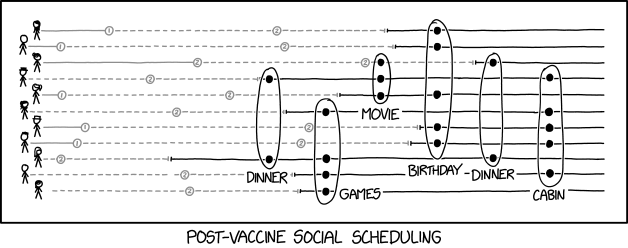
\includegraphics[width=0.8\linewidth]{tex/img/post_vaccine_social_scheduling.png}
	\caption{\emph{As if this problems weren't $\mathcal{NP} $-Hard enough}.
		Post-vaccine social scheduling may be $\mathcal{NP} $-Hard \cite{Munroe}}%
	\label{fig:tex/img/post_vaccine_social_scheduling}
\end{figure}

\paragraph{$\mathcal{NP} $-Complete}%
\label{par:_np_hard} is the set of problems in $\mathcal{NP} $-Hard that are
also in $\mathcal{NP} $. Intuitively these correspond the most difficult
problems to solve in $\mathcal{NP} $. The number of problems which are known to
be in this set is in the order of a thousand \cite{SanjeevArora2017}.

\subsection{$\mathcal{P} $ vs $\mathcal{NP}$}%
\label{sub:_p_vs_np_}

A fundamental question in Computational Complexity is wheter $\mathcal{P} =
	\mathcal{NP} $. Mostly people believe that this is not true, so
$\mathcal{P} \neq \mathcal{NP} $, and also our daily experience tell us that
often it is easier to check the correctness of a solution of a problem than
finding it \cite{9780521884730}: in many cases coming up with the correct
answer requires searching over an exponentially large set
\cite{SanjeevArora2017}. Nonetheless no mathematical proof of this notion has
been found and, in fact, in the last decades there has been little or no progress towards it \cite{Erickson2019}.

If, it is mostly accepted, $\mathcal{P} \neq \mathcal{NP} $ this would produce
a situation as depicted in \autoref{fig:tex/img/complexity-diagram}:
there are problems for which we are not able to find the solution
efficiently (i.e. in polynomial time). On the other side this allows the
existance of one-way-functions (i.e. functions whose inverse is much harder to
compute than the original functions) on which Modern Criptography heavily
relies \cite{9780521884730}.
%
% This brings the need for algorithms which are able to approximate the solution
% in a reasonable amount of time.

% Viceversa, if $\mathcal{P} = \mathcal{NP} $, it would be very easy to find
% proofs and mathematicians could be replaced by
% look at 2.7.3 in Sanjeev's book

\begin{figure}
	\centering
	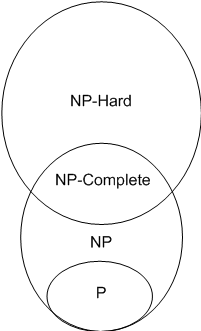
\includegraphics[width=0.3\linewidth]{tex/img/complexity-diagram.png}
	\caption{Venn diagram for the complexity classes if $\mathcal{P} \neq
			\mathcal{NP} $ \cite{article}}%
	\label{fig:tex/img/complexity-diagram}
\end{figure}

\subsection{Optimization Problems and $\mathcal{NPO} $}%
\label{sub:optimization_problems}

Optimization problems are defined from a problem instance $x$, a set of
feasible solutions $S$ and a cost function that takes as input the problem
instance $x$ a feasible solution $s \in S$, denoted as cost$_{O} (x, s) $.
Given a minimization (maximization) problem the optimal solution is defined as
the $s$ minimizing (maximizing) the value of cost$_{O} (x, s)$, and we denote
by opt$_{O} (x) $ this value\cite{Trevisan2004}.

\paragraph{$\mathcal{NPO} $}%
\label{par:_npo_}

is then the set of optimization problems whose cost function
can be computed in polynomial time and for every instance of the problem $x$
and feasible solution for that problem $s \in A$ there is a polynomial $q \; s.t.
	\; s \leq q(|x|)$ (i.e. the size of every solution is bounded by a polynomial
in $x$).

If $\mathcal{P} \neq \mathcal{NP} $ for many optimization problems there is no
algorithm for finding the optimal solution in polynomial time
\cite{Trevisan2004}. This is again a fundamental limitation about what we can
compute which then requires the definition of some alternative approaches, like
the definition of \emph{approximation algorithm}
which are able to be computed in polynomial time
a solution which lies in a given factor from the optimal
one\cite{Vazirani2002}.

\paragraph{Approximation}%
\label{par:r_approximations}

$A$ is an r-approximation algorithm for an $\mathcal{NPO} $ minimization
problem $O$ if, for every instance $x$ of $O$ it holds that
\begin{equation*}
	cost_{O} (x, A(x)) \leq r \cdot opt_{O} (x)
\end{equation*}

\noindent
(or, respectively, cost$_{O} (x, A(x))
	\leq 1/r \cdot $opt$_{O} (x) $ for maximization problems), $A(x)$ being the
optimal solution found by the approximation algorithm \cite{Trevisan2004}.

\subsection{Approximation preserving reductions}%
\label{sub:approximation_preserving_reductions}

Problems approximability varies widely: while for some of them exists
constant factor approximations, for some others even a remotely approximate
solution cannot be found \cite{Ausiello2005} (some examples are listed in
\autoref{tab:inapproximability-examples} ).

% todo: reference to the papers proving each result instead of the hub
\begin{table}
	\centering
	\caption{Examples of known inapproximability results, assuming $\mathcal{P}
			\neq \mathcal{NP} $ \cite{10.1007/3-540-63248-4_10} }
	\label{tab:inapproximability-examples}
	\begin{tabular}{c|p{5cm}|c}
		Problem                                                          & Description                                                   & Inapproximability \\
		\hline
		$ \textsc{MaxClique} $                                           & Biggest complete subgraph                                     & $|V|^{1-
		\epsilon}, \forall \epsilon > 0 $                                                                                                                    \\
		                                                                 &                                                               &                   \\
		$ \textsc{MaximumIndipendentSet} $                               &
		Biggest set of not connected nodes                               & $|V|^{1-
		\epsilon}, \forall \epsilon > 0 $                                                                                                                    \\
		                                                                 &                                                               &                   \\
		$ \textsc{MinCut} $                                              & Partition of nodes in 2 sets $V_1$ and $V_2$ minimizing edges
		between the 2 sets                                               & 1.0624                                                                            \\
		                                                                 &                                                               &                   \\
		$ \textsc{MaximumSetPacking} $                                   & Given a collection of
		finite sets $C$,
		finding the biggest collection $C' \subseteq C$ of disjoint sets & $|C|^{1-
		\epsilon}, \forall \epsilon > 0 $                                                                                                                    \\
	\end{tabular}
\end{table}

\emph{Approximation preserving reductions} are a fundamental notion for proving
a partial order among optimization problems \cite{Ausiello2005}. An
\emph{Approximation preserving reductions} must have
the following properties (when reducing from a problem $A$ to a problem $B$)
\cite{DemaineFall2014}:

\begin{itemize}
	\item any instance $x$ of $A$ should be mapped to an instance $x' = f(x)$
	      of $B$ in polynomial time
	\item any solution $y' \in $ sol$(f(x))$ of $B$ should be associated to a corresponding
	      solution $y = g(x, y') \in $ sol$(x)$ of $A$ in polynomial time
\end{itemize}

So there are 2 efficient (i.e. requiring polynomial time) functions $f$ and $g$
for mapping instances of $A$ to $B$ and solution of $B$ to solutions of $A$,
respectively (\autoref{fig:tex/img/reduction_scheme}).

\begin{figure}
	\centering
	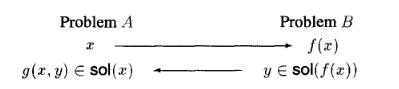
\includegraphics[width=0.6\linewidth]{tex/img/reduction_scheme.png}
	\caption{The reduction scheme \cite{Crescenzi1997ASG}}%
	\label{fig:tex/img/reduction_scheme}
\end{figure}

There are at least 9 different kinds of approximation preserving reductions
\cite{DemaineFall2014}(\autoref{fig:tex/img/approximation_preserving_reductions}) but we will
focus only on one type.

\begin{figure}[b]
	\centering
	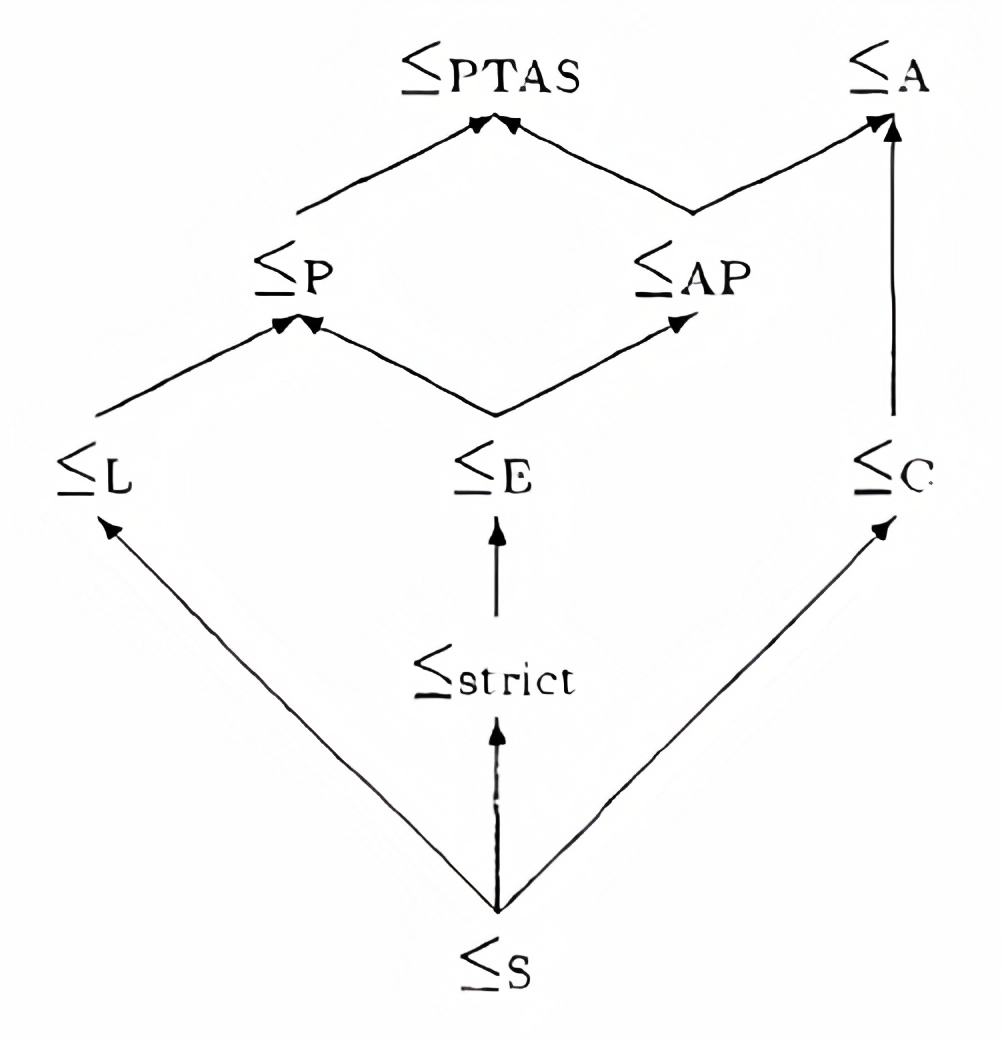
\includegraphics[width=0.4\linewidth]{tex/img/approximation_preserving_reductions.png}
	\caption{Taxonomy of approximation preserving reductions \cite{Crescenzi1997ASG}}%
	\label{fig:tex/img/approximation_preserving_reductions}
\end{figure}

\subsubsection{S reductions}%
\label{sub:strict_reductions}

An $S$ \emph{reduction} from problem $A$ to problem $B$ has the following properties \cite{Crescenzi1997ASG}:
\begin{itemize}
	\item fox any instance $x$ of problem $A$ it holds that opt$_{A} (x) = $ opt$_{B} (f(x))$
	\item for any instance $x$ of $A$ and solution $y'$ of $B$, cost$_{A} (x,
		      g(x, y')) = $ cost$_{B} (f(x), y')$
\end{itemize}

Strict reductions are the strongest type of \emph{approximation preserving
	reductions} and imply all the others \cite{Crescenzi1997ASG}.

\section{Linear and Mixed Integer Programming}%
\label{sec:linear_and_mixed_integer_programming}

\acrlong{LP} is a widely used optimization technique and one of the most
effective; the term refers to problems in which both the constraints and \emph{objective
	function} are linear
\cite{Edgar2001}\cite{Vanderbei2008}\cite{Dantzig1998}\cite{Martin1998}.

\subsection{The structure of a linear programming model}%
\label{sub:the_structure_of_a_linear_programming_model}

In a \acrfull{LP} problem we are given a vector $ \mathbf{c} = (c_1,
	\dots, c_n) $ and we want to maximize (or minimize) a linear function over
the variables $ \mathbf{x} = (x_1, \dots, x_n) $ with the coefficients of the
vector $ \mathbf{c} $, i.e.
\begin{equation*}
	\mathbf{cx} = \sum^{n}_{i=1} c_i x_i
\end{equation*}
(known as the \emph{objective function}) while satisfying some linear
constraints over the variables \cite{Bertsimas1997}\cite{Vanderbei2008}:

\begin{equation*}
	a_1 x_1 + \dots + a_n x_n \begin{Bmatrix} \leq \\ = \\ \geq \end{Bmatrix} b
\end{equation*}

% There is no \emp{a priori} preference regarding how the problem is formulated
% since it is easy to convert an inequality into a equality constraint through
% additional variables ($\omega $ in the example below) called \emph{slack}
% \cite{Vanderbei2008}. For example one in the form
% \begin{equation*}
%     a_1 x_1 + \dots + a_n x_n \leq b
% \end{equation*}
% is equivalent to
% \begin{equation*}
%     a_1 x_1 + \dots + a_n x_n + \omega = b, \quad \omega \geq 0
% \end{equation*}
% and viceversa an equality
% \begin{equation*}
%     a_1 x_1 + \dots + a_n x_n = b
% \end{equation*}
% can be converted into
% \begin{align*}
%     a_1 x_1 + \dots + a_n x_n \leq b \\
%     a_1 x_1 + \dots + a_n x_n \geq b
% \end{align*}
%
In general is possible to formulate any \acrshort{LP} problem as follows (called \emph{standard form}) \cite{Vanderbei2008}

\begin{alignat}{3}
	\label{eq:standard-form}
	\begin{aligned}[t]
		\text{maximize}   &       & \sum_{i=1}^{n} c_{i}x_{i}                                          \\
		\text{subject to} & \quad & \sum_{i=1}^{n} a_{1i}  x_{i} & \leq b_{1} &                        \\
		                  &       & \vdots                                                             \\
		                  &       & \sum_{i=1}^{n} a_{mi}  x_{i} & \leq b_{m} &                        \\
		                  &       & x_{i}                        & \geq 0,    & \quad i & =1 ,\dots, n
	\end{aligned}
\end{alignat}


The $x_i$ are known also as \emph{decision variables}; a choice of $ \mathbf{x}
$ if called \emph{solution} and \emph{feasible solution} if it satisfies the
constraints, \emph{optimum} if it maximizes the \emph{objective function}
\cite{Vanderbei2008}.

\subsection{Solving an LP problem}%
\label{sub:solving_an_lp_problem}

Solving an \acrshort{LP} problem involves a process called the \emph{simplex
	method} which has 2 different phases.

Starting from the \emph{standard form} (\autoref{eq:standard-form})
\emph{slack} variables $x_{n+1}, \dots, $ $x_{n+m} $ are introduced as well as a name
for the \emph{objective} function, allowing to express the problem as follows
\cite{Vanderbei2008}\cite{Edgar2001}

\begin{alignat}{2}
	\label{eq:standard-form}
	 &  & \quad &
	\begin{aligned}[t]
		\zeta   & = \sum_{i=1}^{n} c_{i}x_{i}                                       \\
		x_{n+1} & = b_{1} - \sum_{i=1}^{n} a_{1i}  x_{i} &                          \\
		\vdots                                                                      \\
		x_{n+m} & = b_{m} - \sum_{i=1}^{n} a_{mi}  x_{i} &                          \\
		x_{i}   & \geq 0,                                & \quad i & =1 ,\dots, n+m
	\end{aligned}
\end{alignat}

The first phase involves finding a feasible solution for the problem. More
specifically, we look for $m$ variables, called \emph{basic variables}, whose
value we choose in order to satisfy the $m$ equality constraints (while the
remaining variables, the \emph{nonbasic} ones, are set to 0); if no such
feasible solution exists then the problem is \emph{unfeasible}. Let $\mathcal{B}
$ be the set of \emph{basic variables} and $\mathcal{N} $ the set of
\emph{nonbasic variables} \cite{Vanderbei2008}\cite{Bertsimas1997}. Then the
problem can be reformulated as follows

\begin{alignat}{2}
	\label{eq:standard-form-simplex-new}
	 &  & \quad &
	\begin{aligned}[t]
		\zeta & = \bar{\zeta} + \sum_{j \in \mathcal{N} }^{n} c_{j}x_{j}                                      \\
		x_{i} & = \bar{b}_{i} - \sum_{j \in \mathcal{N} }^{n} \bar{a}_{ij}
		x_{j} & i                                                          & \in \mathcal{B}                  \\
		x_{i} & \geq 0,                                                    & \quad i         & =1 ,\dots, n+m
	\end{aligned}
\end{alignat}

The second phase of the \emph{simplex method} aims at improving the current
solution: if $c_{j} \geq 0, \; \forall j \in \mathcal{N} $ then the value of the
objective function cannot be increased and we found an optimum. If, instead, there is at least a $c_{j}
	> 0$ then we can increase the value of $\zeta$ by increasing $x_{j} $; now
there are 2 different cases \cite{Vanderbei2008}
\begin{itemize}
	\item as $x_{j} $ increases there is at least a variable $\tilde{x}_{j} $
	      whose value needs to decrease to satisfy equality constraints. The first
	      of these variables $\tilde{x}_{j} $ reaching to $0$ moves from
	      $\mathcal{B} $ to $\mathcal{N} $, while
	      $x_{j} $ moves from $\mathcal{N} $ to $\mathcal{B} $. The problem is reformulated again as in
	      \autoref{eq:standard-form-simplex-new} and the process is repeated
	      \cite{Vanderbei2008}.
	\item if no such $\tilde{x}_{j} $ variable exists then the value of $x_{j}
	      $ can be increased indefinitely and the problem is said to be
	      \emph{unbounded}, i.e. it can achieve any arbitrarily large value.
\end{itemize}

The process is illustrated in \autoref{fig:tex/img/simplex}.

\begin{figure}
	\centering
	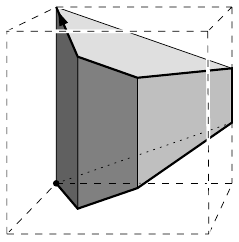
\includegraphics[width=0.4\linewidth]{tex/img/simplex.png}
	\caption{An example of the progress of the \emph{simplex method}: the
		process moves along the vertices of the polygon defined by the
		contraints while improving the value of the solution \cite{BerndGaertner2006}}%
	\label{fig:tex/img/simplex}
\end{figure}

\subsection{Mixed Integer Programming}%
\label{sub:mixed_integer_programming}

Many problems involve not only continous variables but also variable that take binary or
integer values: these are known as \acrfull{MIP} problems. Furthermore, some of
these problems are linear in the constraints and objective function and are
known as \acrfull{MILP} problems
\cite{Edgar2001}\cite{Wolsey1998}.

A generic \acrshort{MILP} can be expressed as \cite{Conforti2016}

\begin{alignat}{3}
	\label{eq:standard-form-milp}
	\begin{aligned}[t]
		\text{maximize}   &                                     & \sum_{i=1}^{n_{1} } c_{i}x_{i} +
		\sum_{i=1}^{n_{2} } h_{i}y_{i}                                                                                                                               \\
		\text{subject to} & \quad                               & \sum_{i=1}^{n_{1} } a_{1i}  x_{i} + \sum_{i=1}^{n_{2} } g_{1i}  y_{i} & \leq b_{1}       &         \\
		                  &                                     & \vdots                                                                                             \\
		                  &                                     & \sum_{i=1}^{n_{1} } a_{mi}  x_{i} + \sum_{i=1}^{n_{2} } g_{1i}  y_{i} & \leq b_{m}       &         \\
		% &       & \sum_{i=1}^{n} a_{mi}  x_{i}                                          & \leq b_{m} &                        \\
		                  &                                     & x_{i}
		                  & \geq 0,                             & \quad i                                                               & =1 ,\dots, n_{1}           \\
		                  &                                     & y_{i}                                                                 & \geq 0,          & \quad i
		                  & =1 ,\dots, n_{2} \; \text{integral}
	\end{aligned}
\end{alignat}

For convenience we will refer to \acrshort{MILP} problems as \acrshort{MIP} in
the rest of the document.

The \emph{relaxation} of a \acrshort{MIP} problem is defined as the same
problem where the integrality constraints have been removed \cite{Edgar2001}.

Solving a \acrshort{MILP} is a difficult task in general, differently from the
\acrshort{LP} problems. It has been shown also that \acrshort{MIP} is
$\mathcal{NP}$-\textbf{Hard}
\cite{Kannan1978}\cite{Liberti2019}\cite{Schrijver1998}. This is why the \emph{relaxation} is often considered
to get an approximation of the exact solution and it is much easier
\cite{Conforti2016}.

\subsection{Solving a MIP}%
\label{sub:solving_a_mip}

One approach that has been proven successfull for solving \acrshort{MIP} is th
e Branch-and-Bound, which is guaranteed to find an optimal solution
\cite{Conforti2016}\cite{Edgar2001}.

Given a problem $P$ the process starts by solving the \emph{relaxation} of $P$
and finding its optimal solution $(\tilde{x}, \tilde{y})$.
Let $S$ and  $\tilde{S}$ be the set of feasible solutions
for the original problem $A$ and its relaxation, respectively. By definition
we have that $S \subseteq \tilde{S} $.
Therefore \cite{Edgar2001}
\begin{itemize}
	\item If the relaxation problem is not feasible so will also the original
	      problem
	\item If $\tilde{y}$ has only integer values then we found the optimal
	      solution for the original problem $A$
\end{itemize}

If, instead, $\tilde{y}$ contains some fractional values, we start by
initialing the value of the best solution so far, $\zeta$, with $-\infty$.
Then we choose one of the fractional variables that are required to be integral
in the original problem $A$, say $y_j$ with value $f$, and create $2$
subproblems, respectively adding the constraint $y_{j} \leq \lfloor f \rfloor$
and $y_{j} \geq \lceil f \rceil$. This step is called \emph{branching}. We now
consider the solution of each subproblem $(x_j, y_j)$ with value of the
objective function $z_{j} $ \cite{Edgar2001}\cite{Conforti2016}.

\begin{itemize}
	\item If either of the subproblems is not feasible or its value $z_{j} $ is
	      lower then the best one found so far then it does not to be
	      considered further. This is called \emph{pruning}.
	\item otherwise if $y_{j} $ are all integer values then $\zeta = z_{j} $
	\item otherwise we subdivide again in $2$ subproblems as done above.
\end{itemize}

When there are no remaining subproblems to consider the Branch-and-Bound method
terminates \cite{Edgar2001}.

\section{Related work}%
\label{sec:related_work}

\cleardoublepage

% \chapter{Methods}
\label{ch:methods}

This chapter focuses on describing the main topic of the
research: the problems are motivated and defined in
\autoref{sec:the_echo_chamber_problem}, and their complexity is then analyzed
in \autoref{sec:problem_complexity_and_approximability}, while proposing some
alternative problem definitions. Algorithms and models for solving and
approximating the problems are then proposed in
\autoref{sec:solving_the_problem}; the definition of a generative model
concludes the chapter (\autoref{sec:generative_model}).

\section{The \acrlong{ECP}}%
\label{sec:the_echo_chamber_problem}

This section starts by outlining the graph on which the analysis is carried
out (\autoref{sub:interaction-graph}), the process for building it
(\autoref{sub:collection_and_preprocessing}) and finally defines the
\acrlong{ECP} and the \acrlong{D-ECP} (\autoref{sub:the_problem_definition} and
\autoref{sub:the_densest_echo_chamber_problem}).

\subsection{The Interaction Graph}
\label{sub:interaction-graph}

The \emph{Interaction Graph} $G$ is the graph which encodes the informations
regarding the interactions between the users.

In this graph each users is associated to a vertex $v \in V$ and each edge to
an interaction between the $2$ corresponding users it links. For this reason we
will sometime refer to vertices as users in the rest of the document.

$G = (V, E^{+}, E^{-})  $ is a
signed and weighted graph, the weights being in the interval $[-1, +1]$,
corresponding to positive and negative interactions, meaning that for smaller
the value of the weight the interaction will more "negative".

The \emph{Interaction Graph} is also directed, so that an edge from vertex $v_{i}
$ to vertex $v_{j} $ corresponds to a reply from user $v_{i} $ to $v_{j} $.

Let a content $C$ be any kind of resource that triggers a discussion in one or
more threads $T$. The set of threads associated to $C$ is denoted as
$\mathcal{T}_{C} $. A content is usually represented by a newspaper article and
it is identified by its url, e.g.

	{\footnotesize
		\begin{center}
			\url{https://www.nytimes.com/2021/03/04/us/richard-barnett-pelosi-tantrum.html}
		\end{center}
	}

A corresponding thread may then be, for example, a user posting and commenting
the same url on its Twitter account (see \autoref{fig:twitter-thread}), thus
generating a discussion.

\begin{figure}
	\centering
	
\includegraphics[width=0.6\linewidth]{tex/img/twitter_thread.png}
	\caption[Thread-content distinction example from Twitter]{An thread associated to the mentioned New York Times article}%
	\label{fig:twitter-thread}
\end{figure}

The \emph{Interaction Graph} is a \emph{multiplex graph}, each layer being
represented by a thread $T$ whose edges are the interactions happening in it.
Note also that for this reason each of the layers can contain more than one
edge between $2$ users, as each pair of users can reply to each other more than
once.

We will also use $\mathcal{C} $ for denoting the set of contents.

An example of \emph{Interaction Graph} can be seen in
\autoref{fig:interaction-graph-example}.

\begin{figure}
	\begin{center}
		\begin{subfigure}[b]{0.3\textwidth}
			\centering
			\tikzfig{tex/tikz/graph_thread1}
			\caption{$T_{1} \in \mathcal{T}_{C_{1}} $}
			\label{fig:tex/tikz/graph_thread1.tikz}
		\end{subfigure}
		\begin{subfigure}[b]{0.3\textwidth}
			\centering
			\tikzfig{tex/tikz/graph_thread2}
			\caption{$T_{2} \in \mathcal{T}_{C_{1}} $}
			\label{fig:tex/tikz/graph_thread2.tikz}
		\end{subfigure}
		\begin{subfigure}[b]{0.3\textwidth}
			\centering
			\tikzfig{tex/tikz/graph_thread3}
			\caption{$T_{3} \in \mathcal{T}_{C_{2}} $}
			\label{fig:tex/tikz/graph_thread3.tikz}
		\end{subfigure}
	\end{center}
	\caption[Example \emph{Interaction Graph}]{An example of \emph{Interaction Graph}, green and red edges
		representing positive and negative interactions, respectively. It
		contains $3$ threads and $2$ contents, the first $2$ layers each being
		associated to a thread of content $C_{1} $, the last layer to a thread
		of content $C_{2} $}
	\label{fig:interaction-graph-example}
\end{figure}

\subsection{Collection and preprocessing}%
\label{sub:collection_and_preprocessing}

Datasets are built mainly upon $2$ social medias: Twitter and Reddit; the data
collection process, consequently, slightly differ between them.

\paragraph{Twitter}%
\label{par:twitter-data}

Twitter's \emph{Interaction Graphs} are mainly built starting from the tweets
of some important social accounts associated to well-known news source, like The
New York Times or Fox News, that tipically post links to their articles:
these profiles are taken as the source of the contents $\mathcal{C} $ of the graph.

Each time another user tweets the same url (\autoref{fig:twitter-thread}) then
it will correspond to another thread related to the same content, and all the
replies it receives will be part of this new thread.

Twitter data is retrieved with the help of Tweepy \cite{tweepy}, a Python
library for accessing the Twitter API, which has been patched for using some
features available only in the beta of the new Twitter API (v2).

\paragraph{Reddit}%
\label{par:reddit}

Differently from Twitter, Reddit focuses on subreddits, which are pages
collecting posts from different users about a specific topic (e.g. r/politics,
r/economics, $\dots$). This means that
in the datasets built from this social media the contents $\mathcal{C} $ is the
set of posts of these pages, which, differently from Twitter, most likely
come from different sources.

This posts are in turn crossposted, i.e. reposted on other subreddits. Each of
these \emph{crosspost} will eventually correspond to another thread.

The PRAW library is used for retrieving the data \cite{praw}.

\paragraph{Edge weights assignment}%
\label{par:assigning_edge_weights}

Once the threads interactions are retrieved they are passed to a state of the
art sentiment analyzer which labels them. More specifically the model used is
RoBERTa which has been adapted and retrained for dealing with Twitter
data \cite{Barbieri2020}. The model is made available by the Transformers
python library \cite{wolf-etal-2020-transformers}.

\bigskip

Finally, complying with the current privacy legislation, all the data related
to the user is pseudo-anonymized (accounts identifier are replaced by random
ones) while no data is publicly available.

\subsection{The problem definition}%
\label{sub:the_problem_definition}

The main goal of the research is finding echo chambers in social medias, more
specifically on the \emph{Interaction Graph} as defined in
\autoref{sub:interaction-graph}.

Our definition is based on the idea that echo chambers can be identified by
looking at contents which is generally highly debated (we will call
this type of content \emph{controversial}) but which is discussed with little
or no animosity in small subgraphs. This subgraphs are the \emph{Echo
	Chambers}.

\bigskip

Given an \emph{Interaction Graph} $G = (V, E^{+}, E^{-})$ on some contents
$\mathcal{C} $ and threads, let $\eta(T)$ the number of negative edges over the
total number of edges in the layer associated to thread $T$. Similarly,
let $\eta(C)$ be the fraction of negative edges in all threads associated to
content $C$.

\begin{definition}[Controversial thread]
	Let $\alpha \in [0,1]$. A thread (or content) is \emph{controversial} if
	$\eta(T) > \alpha$ (or, similarly, $\eta(C) > \alpha $). Conversely, a
	thread (or content) is \emph{non-controversial} if $\eta(T) \leq \alpha$
	($\eta(C) \leq \alpha$).
\end{definition}

Intutively, \emph{controversial} threads contain many negative
interactions. We denote as $\hat{\mathcal{C} } \subseteq \mathcal{C} $ the
set of \emph{controversial} contents.

\medskip

\emph{Echo Chambers} correspond to \emph{non-controversial} smaller subgraphs
(i.e. with few negative edges) discussing a
\emph{controversial} content.

More formally, let $T[U]$ the subgraph induced in the layer associated to
thread $T$ by the vertices $U$; let $|T^{+} [U]|$ and $|T^{-} [U]|$ its number
of positive and negative edges, respectively.

We define $\mathcal{S}_C (U)$ as the set of \emph{non-controversial} threads
induced by $U$, for \textit{controversial} contents, i.e.
	{\small
		\begin{equation}
			\mathcal{S} _{C} (U) = \{ T[U] \; s.t. \; T[U] \; non \;
			controversial, T \in \mathcal{T} _{C}, C
			\in \hat{\mathcal{C}}, U \subseteq V\}
		\end{equation}
	}

Thus $\mathcal{S} _C (U)$ will contain threads which are \emph{globally} non
controversial but it is defined only for contents that are \emph{globally}
controversial.

\medskip

We know define the Echo Chamber Score of a set of vertices $U$.

\begin{definition}[Echo Chamber Score]
	Let $U \subseteq V$ be a subset of vertices. Its Echo Chamber Score is

	\begin{equation}
		\label{eq:echo-chamber-score}
		\xi(U) = \sum^{}_{\mathcal{C} \in \mathcal{\hat{C}}} \sum^{}_{T[U] \in
		\mathcal{S} _{C} (U)} (|T^{+} [U]| - |T ^{-} [U]|)
	\end{equation}
\end{definition}

We can now define the \acrfull{ECP}.

\begin{problem}[\acrfull{ECP}]
Given an \emph{Interaction Graph} $G$ and $\alpha \in [0, 1]$ find a set of vertices $U \subseteq
	V$ maximizing the Echo Chamber Score (\autoref{eq:echo-chamber-score}).
\end{problem}

We will denote with $\hat{U}$ the set of users maximizing
\autoref{eq:echo-chamber-score} and with $\xi(G)$ its corresponding score, i.e.

\begin{align*}
	\hat{U} & \coloneqq \argmax_{U \subseteq V} \xi(U) & \xi(G) & \coloneqq
	\xi(\hat{U})
\end{align*}

\subsection{The Densest Echo Chamber Problem}%
\label{sub:the_densest_echo_chamber_problem}

The \acrshort{ECP} doesn't take into account the number of users producing a
certain score; this means that the set $U$ may involve disconnected and sparse
subgraphs, depending on the structure of the graph $G$.

For this reason it is interesting also to study another variant of the
\acrshort{ECP}, the \acrlong{D-ECP}, which we now define.

\begin{definition}[Echo Chamber Score]
	Let $U \subseteq V$ be a subset of vertices. Its Densest Echo Chamber Score is

	\begin{equation}
		\label{eq:densest-echo-chamber-score}
		\xi(U) = \sum^{}_{\mathcal{C} \in \mathcal{\hat{C}}} \sum^{}_{T[U] \in
		\mathcal{S} _{C} (U)} \frac{(|T^{+} [U]| - |T ^{-} [U]|)}{|U|}
	\end{equation}
\end{definition}

Similarly to the \acrshort{ECP} we can now define the corresponding problem

\begin{problem}[\acrfull{D-ECP}]
Given an \emph{Interaction Graph} $G$ and $\alpha \in [0, 1]$ find a set of vertices $U \subseteq
	V$ maximizing the Densest Echo Chamber Score (\autoref{eq:densest-echo-chamber-score}).
\end{problem}

\section{Problems complexity and approximability}%
\label{sec:problem_complexity_and_approximability}

We will now prove the inapproximability of the \acrshort{ECP} and
\acrshort{D-ECP} within some nontrivial factor.

\subsection{Hardness of \acrshort{ECP}}%
\label{sub:ecp-hardness}

\begin{theorem}
	\label{th:approximability}
	Echo Chamber Problem (ECP) has no $n^{1-\epsilon} $-approximation algorithm for
	any $\epsilon$ unless $\mathcal{P} = \mathcal{NP}  $
\end{theorem}

\begin{proof}
	We show this by presenting a direct reduction from \textsc{Maximum
		Independent Set} (MIS), which is known having the mentioned hardness
	factor (\autoref{tab:inapproximability-examples}).

	\bigskip
	Let $G_{1}  = (V_{1} ,E_{1} )$ be an undirected and unweighted graph and
	$\lambda > \frac{\alpha }{1 - \alpha }$, $\lambda \in \mathbb{N} $ and $n_{1} \coloneqq |V_{1}| $.
	We construct the \emph{Interaction Graph} ${G}_{2}  = (V_{2} , E^{+}_{2} , E
			^{-}_{2} ) $ as follows

	\begin{itemize}
		\item for each vertex $v_{i}  \in V_{1} $ we add a vertex in $G_{2} $
		\item for each edge $e_{ij}  \in
			      E_{1} $ we add $\lambda n_{1} $ negative edges between $v_{i} $ and $v_{j} $
		\item add a vertex $v_r$ and a positive edge between it and any other
		      vertex that we already inserted in $G_2$
		\item add a vertex $v_x$ and $\lambda n_{1} $ negative edges between $v_x$
		      and $v_{r} $
	\end{itemize}

	Furthermore, all the edges in $G_{2} $ are associated to the same content
	$C$ and the same thread $T \in \mathcal{T}_{C}  $.
	An illustration of the conversion can be found in \autoref{fig:construction}.

	\begin{figure}[b]
		\begin{center}
			\begin{subfigure}{0.4\textwidth}
				\centering
				\tikzfig{tex/tikz/approximability1}
				\vspace{10pt}
				\caption{$G_{1}$, undirected graph}
				\label{fig:g1_example}
			\end{subfigure}
			\begin{subfigure}{0.4\textwidth}
				\centering
				\tikzfig{tex/tikz/approximability2}
				\caption{$G_{2}$, directed signed graph, for $\lambda = 1$}
				\label{fig:g2_example}
			\end{subfigure}
		\end{center}
		\caption[Example reduction from MIP to \acrshort{ECP}]{Example construction of the interaction graph $G_{2} $ from
			$G_{1} $, for $\alpha = \frac{1}{2} $}
		\label{fig:construction}
	\end{figure}

	\begin{claim}
		\label{th:claim-controversial}
		Content $C$ is controversial.
	\end{claim}
	\begin{proof}
		Let $m_{2}^{-} $ and $m_{2}^{+} $ be the number of negative and
		positive edges in $G_2$, respectively.

		By construction $m_{2}^{+} = n_{1} $ and $m_{2}^{-} \geq \lambda n_{1}
		$. Also, for $a, b, c \in \mathbb{R}^{+}$ it holds that $\frac{a +
				b}{a + b + c} \geq \frac{a}{a + c} $. Consequently

		\begin{align}
			\eta(C) = \frac{m_{2}^{-} }{m_{2}^{-} +
				m_{2}^{+} } \geq \frac{\lambda n_{1}}{\lambda n_{1}
				+ n_{1} } = \frac{\lambda }{\lambda + 1} > \alpha
		\end{align}
	\end{proof}

	So content C is controversial. This reduces the Echo Chamber Problem on $G_2$ to the maximization of

	\begin{equation}
		\label{eq:score}
		\xi(U) = \sum^{}_{T \in S_{C}(U) } | T[U] |
	\end{equation}

	\begin{claim}
		\label{th:opt-equality}
		\begin{equation}
			OPT(ECP) = OPT(MIS)
		\end{equation}
	\end{claim}

	\begin{proof}
		Let $I \subseteq V_{1} $ be an independent set of $G_1$ of size $|I| >
			1$. Consider the associated solution in $G_2$ in which $U = I
			\cup \{v_{r} \}$. By construction it will contain $|I|$ positive
		edges, so $T$ will not be controversial and also

		\begin{equation}
			OPT(ECP) \geq \xi(U) = |T[U]| = |I| \implies OPT(ECP) \geq OPT(MIS)
		\end{equation}

		Now let $S \subseteq V_2$ be a solution of the Echo Chamber problem on
		$G_2$, and suppose $\xi(S) > 0$. It is easy to see that $v_{r} \in S$
		and that $v_{x} \not\in S $. Let $J \coloneqq S \setminus \{v_r\}$.

		Suppose that $2$ vertices $v_{i} $, $v_{j} \in J$ are linked in
		$G_1$. By construction there are at least $\lambda n_1$ negative edges
		in $T[S]$, thus

		\begin{equation}
			\eta(T[S]) \geq \frac{\lambda n_1}{\lambda n_1 + |S-1|} \geq \frac{\lambda n_1}{\lambda n_1 + n_1} = \frac{\lambda
			}{\lambda + 1} > \alpha
		\end{equation}

		This means that $T[S]$ is controversial $\implies \xi(S) = 0
			\implies contradiction$. Consequently $J$
		contains vertices which are independent in $G_1$. Therefore $T[S]$ contains
		only positive edges; more specifically

		\begin{equation}
			\xi(S) = |T[S]| = |S| - 1 = |S \setminus \{v_r\}| = |J|
		\end{equation}

		Thus

		\begin{equation}
			OPT(MIS) \geq |J| \implies OPT(MIS) \geq OPT(ECP)
		\end{equation}

		So the optimal value of the constructed instance of Echo Chamber Problem
		exactly equals that of the \textsc{Maximum Independent Set} instance, so it
		has an hardness factor at least as large as that of MIS.
	\end{proof}

	This concludes the proof of \autoref{th:approximability}.
\end{proof}

\subsection{Hardness of \acrshort{D-ECP}}%
\label{sub:d-ecp-hardness}

\begin{theorem}
	\label{th:approximability-densest}
	Densest Echo Chamber Problem (D-ECP) has no $n^{1-\epsilon} $-approximation algorithm for
	any $\epsilon$ unless $\mathcal{P} = \mathcal{NP}  $
\end{theorem}

\begin{proof}
	We again show this by presenting a direct reduction from \textsc{Maximum
		Independent Set}.

	\bigskip
	Let $G_{1}  = (V_{1} ,E_{1} )$ be an undirected and unweighted graph and
	$\lambda > \frac{\alpha }{1 - \alpha }$, $\lambda \in \mathbb{N} $ and $n_{1} \coloneqq |V_{1}| $.
	We construct the \emph{interaction} graph ${G}_{2}  = (V_{2} , E^{+}_{2} , E
			^{-}_{2} ) $ as follows

	\begin{itemize}
		\item for each vertex $v_{i}  \in V_{1} $ we add a vertex in $G_{2} $
		\item for each edge $e_{ij}  \in
			      E_{1} $ we add $\lambda (n_{1}+1)^{2}  $ negative edges between $v_{i} $ and $v_{j} $
		\item for each edge $e_{ij} \in V_1 \times V_1, e_{ij} \not\in
			      E_{1} $ we add $2$ positive edges between $v_{i} $ and $v_{j} $
		\item add a vertex $v_r$ and $2$ positive edges between it and any other
		      vertex that we already inserted in $G_2$
		\item add a vertex $v_x$ and $\lambda n_{1}^{2}  $ negative edges between $v_x$
		      and $v_{r} $
	\end{itemize}

	Furthermore, all the edges in $G_{2} $ are associated to the same content
	$C$ and the same thread $T \in \mathcal{T}_{C}  $.
	An illustration of the conversion can be found in
	\autoref{fig:construction-densest}.

	\begin{figure}
		\begin{center}
			\begin{subfigure}[b]{0.4\textwidth}
				\centering
				\tikzfig{tex/tikz/approximability1-densest}
				\vspace{30pt}
				\caption{$G_{1}$, undirected graph}
				\label{fig:g1_example}
			\end{subfigure}
			\begin{subfigure}[b]{0.4\textwidth}
				\centering
				\tikzfig{tex/tikz/approximability2-densest}
				\caption{$G_{2}$, directed signed graph}
				\label{fig:g2_example}
			\end{subfigure}
		\end{center}
		\caption[Example reduction from MIP to \acrshort{D-ECP}]{Example construction of the interaction graph $G_{2} $ from
			$G_{1} $}
		\label{fig:construction-densest}
	\end{figure}

	\begin{claim}
		\label{th:claim-controversial-densest}
		Content $C$ is controversial.
	\end{claim}
	\begin{proof}
		% Let $m_{2}^{-} $ and $m_{2}^{+} $ be the number of negative and
		% positive edges in $G_2$, respectively.
		%
		By construction $m_{2}^{+} \leq n_{1}^{2}  $ and $m_{2}^{-} \geq
			\lambda n_{1}^{2} $.
		Thus

		\begin{align}
			\eta(C) = \frac{m_{2}^{-} }{m_{2}^{-} +
				m_{2}^{+} } \geq \frac{\lambda n_{1} ^{2} }{\lambda n_{1}^{2}
				+ n_{1}^{2}  } = \frac{\lambda }{\lambda + 1}
			> \alpha
		\end{align}
	\end{proof}

	So content C is controversial. This reduces the Densest Echo Chamber Problem on $G_2$ to the maximization of

	\begin{equation}
		\label{eq:score-densest}
		\psi(U) = \sum^{}_{T \in S_{C}(U) } \frac{| T[U] |}{|U|}
	\end{equation}

	\begin{claim}
		\label{th:opt-equality-densest}
		\begin{equation}
			OPT(D-ECP) = OPT(MIS)
		\end{equation}
	\end{claim}

	\begin{proof}
		Let $I \subseteq V_{1} $ be an independent set of $G_1$ of size $n_{I}
			\coloneqq |I| > 1$. Consider the associated solution in $G_2$ in
		which $U = I \cup \{v_{r} \}$.

		By construction it will contain
		\begin{itemize}
			\item $2 \cdot n_{I} $ positive edges between $v_{r} $ and $v_{i} \in I$
			\item $n_{I}(n_{I}  -1)$
			      positive edges between vertices $v_{i} \in I$

		\end{itemize}
		$|I|$ positive
		thus $T$ will not be controversial and also

		\begin{equation}
			\label{eq:score-densest-mip}
			\psi(U) = \frac{|T[U]|}{|U|}  = \frac{2n_{I}  +
				\cdot n_{I}(n_{I}  -1) }{n_{I} + 1} = \frac{n_{I}^{2} +
				n_{I}}{n_{I} + 1} = n_{I}
		\end{equation}

		Consequently

		\begin{equation}
			OPT(D-ECP) \geq \psi(U) = |I| \implies OPT(D-ECP) \geq OPT(MIS)
		\end{equation}

		Now let $S \subseteq V_2$ be a solution of the Densest Echo Chamber
		problem on $G_2$, and suppose $\psi(S) > 0$. It is easy to see that
		$v_{r} \in S$ and that $v_{x} \not\in S $. Let $J \coloneqq S \setminus
			\{v_r\}$.

		Suppose that $2$ vertices $v_{i} $, $v_{j} \in J$ are linked in $G_1$.
		By construction there are at least $\lambda (n_1 + 1)^{2} $ negative edges in
		$T[S]$, thus

		\begin{equation}
			\eta(T[S]) \geq \frac{\lambda (n_1+1)^2}{\lambda (n_1+1)^2 + n(n+1)} \geq
			\frac{\lambda (n_1+1)^{2} }{\lambda (n_1+1)^2 + (n_1+1)^2} = \frac{\lambda }{\lambda +
				1} > \alpha
		\end{equation}

		This means that $T[S]$ is controversial $\implies \psi(S) = 0
			\implies contradiction$. Consequently $J$
		contains vertices which are independent in $G_1$. Therefore $T[S]$ contains
		only positive edges. As shown previously in
		\autoref{eq:score-densest-mip}

		\begin{equation}
			\psi(S) = \frac{|T[S]|}{|S|} = |J|
		\end{equation}

		Thus

		\begin{equation}
			OPT(MIS) \geq |J| \implies OPT(MIS) \geq OPT(D-ECP)
		\end{equation}

		So the optimal value of the constructed instance of Densest Echo Chamber Problem
		exactly equals that of the \textsc{Maximum Independent Set} instance, so it
		has an hardness factor at least as large as that of MIS.
	\end{proof}

	This concludes the proof of \autoref{th:approximability-densest}.
\end{proof}

\section{Solving the problem}%
\label{sec:solving_the_problem}

Now we present some techniques for calculating exactly and approximating both
the \acrshort{ECP} and the \acrshort{D-ECP}.

\subsection{A MIP model for the \acrshort{ECP}}%
\label{sub:a_mip_model_for_the_ecp}

Let $G$ be our \emph{Interaction Graph} for contents $\mathcal{C} $,
controversial contents $\mathcal{\hat{C}} \subseteq \mathcal{C} $ and
threads $T \in \mathcal{T}_{C}, \; C \in \mathcal{C} $. Let $E_k$ bet the set
of all edges of thread $T_k$ associated to a controversial content, i.e. $T_{k}
	\in \mathcal{T}_{C}, C \in \mathcal{\hat{C}}$; let also $E^{+}_k $
and $E^{-}_k $ be the set its positive and negative edges, respectively. Fix $\alpha \in [0, 1]$.

The following \acrshort{MIP} model is able to solve the \acrshort{ECP} on $G$
for values of $\alpha \leq 0.5$.

\begin{equation}
	\label{eq:ecp-exact1}
	\text{maximize} \; \sum_{ T_{k} \in \mathcal{T}_{C}, \; C \in
		\mathcal{\hat{C}} } \big( \sum^{}_{ij \in E^{+} (T_{k})} x_{ij}
		^{k} - \sum_{ij \in E^{-} (T_{k})} x_{ij} ^{k} \big)
\end{equation} \begin{center} subject to \end{center}
\begin{gather}
	\label{eq:ecp-v1}
	x _{ij}^{k}  \leq y_i \quad\quad \forall ij \in E_k  \\
	\label{eq:ecp-v2}
	x _{ij}^{k}  \leq y_j \quad\quad \forall ij \in E_k \\
	\label{eq:ecp-t1}
	x _{ij}^{k}  \leq z_k \quad\quad \forall ij \in E_k \\
	\label{eq:ecp-e1}
	x _{ij} ^{k} \geq - 2 + y_i + y_j + z_k \quad\quad \forall ij \in E_k \\
	\label{eq:ecp-alpha-constraint1}
	\sum^{}_{ij \in E_k^{-} } x_{ij}^{k}  - \alpha \sum^{}_{ij \in E_k}
	x_{ij} ^{k}  \leq 0 \quad\quad \forall T_{k} \in \mathcal{T} _{C}, C \in
	\hat{\mathcal{C}} \\
	\label{eq:ecp-vertex-def1}
	y _{i} \in  \{0, 1\} \quad\quad \forall i \in V \\
	\label{eq:ecp-edge-def1}
	0 \leq x _{ij} ^{k}  \leq 1 \quad\quad \forall ij \in E_k \\
	\label{eq:ecp-thread-def1}
	0 \leq z _{k} \leq 1 \quad\quad \forall T_{k} \in \mathcal{T} _{C}, C \in
	\hat{\mathcal{C}}
\end{gather}

The \acrshort{MIP} model introduces variables $x$, $y$ and $z$.
\begin{itemize}
	\item $y$ variables are associated to vertices
	      (\autoref{eq:ecp-vertex-def1}). Intutively $y_i = 1$ means that the
	      vertex $v_{i} $ is part of the set $U \subseteq V$ considered for the
	      score. Let $U \coloneqq \{ v_{i} \; s.t. \; y_{i} = 1, \;
		      v_{i} \in V \}$.
	\item $x$ variables are associated to edges (\autoref{eq:ecp-edge-def1}).
	      A value of $x_{ij}^{k} = 1$ should be interpreted as the fact that
	      the edge $e_{ij} \in E_k$ is contributing to the score,
	      i.e. $T_k \in \mathcal{S}_{C} (U)$.
	\item $z$ variables are associated to threads
	      (\autoref{eq:ecp-thread-def1}). A value of $1$ in this case
	      is associated to \emph{non-controversial} threads.
\end{itemize}

Let us consider Equations \ref{eq:ecp-v1}-\ref{eq:ecp-t1}. Due to them an
edge $e_{ij} \in E_k $ implies that
both vertices $v_{i} $ and $v_{j} $ are in $U$ and the thread is not controversial.

Viceversa \autoref{eq:ecp-e1} makes sure that, if both the incident vertices
are in $U$ and $z_{k} = 1$, then the edge contributes to the score.

Let us now consider a thread $T_k \in \mathcal{S}_{C} $.

Due to \autoref{eq:ecp-t1} and \autoref{eq:ecp-e1} all and only the edges
induced by $U$ have value $z_{k} $, i.e. $x_{ij}^{k} = z_k \; \forall v_{i}, v_{j}
	\in U$.

These variables will contribute to the objective function by

\begin{equation}
	\label{eq:ecp-thread-contribution}
	\sum^{}_{ij \in E^{+}_k } x_{ij} ^{k} - \sum_{ij \in E^{-} _k}
	x_{ij} ^{k} = \sum^{}_{ij \in E^{+} _k} z_k - \sum_{ij \in E^{-} _k}
	z_k = z_k (|E^{+} _k| - |E^{-} _k|)
\end{equation}

Let's suppose $T_k$ \emph{non-controversial}. Then by definition we have
$\eta(T_k) \leq \alpha $ and so

\begin{align}
	\eta(T_k)                                  & \leq \alpha        \\
	\frac{|E^{-} _k|}{|E^{-} _k| + |E^{+} _k|} & \leq \alpha        \\
	{|E^{-} _k|}                               & \leq \alpha(|E^{-}
	_k| + |E^{+} _k|)                                               \\
	\alpha {|E^{+} _k|}                        & \geq (1 -
	\alpha ) |E^{-} _k|                                             \\
	\frac{{|E^{+} _k|}}{|E^{-} _k|}
	                                           & \geq \frac{(1 -
		\alpha )}{\alpha } \geq 1
\end{align}

Where the last inequality holds since $\alpha \in [0, 0.5]$. So $|E^{+} _k| \geq
	|E^{-} _k|$. Thus the contribution of the thread will be maximized by
choosing $z_k = 1$ (\autoref{eq:ecp-thread-contribution}).
\autoref{eq:ecp-alpha-constraint1} can be easily seen to be satisfied since the
thread is \emph{non-controversial}.

Let us now suppose that $T_k \not\in \mathcal{S}_{C}(U)  $ . In this case setting $z_k$ to a value
different from $0$ will violate constraint~\ref{eq:ecp-alpha-constraint1}.

\bigskip

Let us now consider $\alpha \in (0.5, 1]$. With the current formulation if, for
a thread $T_k$, we have that $0.5 < \eta(T_k) \leq \alpha $ then the model will
prefer a solution in which all the edges $e_{ij} \in E_k$ are set to $0$, which
still satisfies all the constraints, even if the induced subgraph in the thread
is \emph{non-controversial} (and so contributes to the score and $x_{ij}^{k}  $
need to be set to 1). For this reason we need to introduce to the previous
problem the following constraints

\begin{gather}
	\label{eq:ecp-a-alpha-constraint}
	\sum^{}_{ij \in E^{-} (T_k)} a_{ij}^{k}  - \alpha \sum^{}_{ij \in E(T_k)}
	a_{ij} ^{k} \geq - N_{k} z_{k}  \quad\quad \forall T_{k} \in \mathcal{T} _{C}, C \in
	\hat{\mathcal{C}} \\
	\label{eq:ecp-a-ij-g-i-j}
	a_{ij}^{k} \geq -1 + y_i + y_j \quad\quad \forall ij \in E_k \\
	\label{eq:ecp-a-ij-l-i}
	a_{ij}^{k} \leq y_i\quad\quad \forall ij \in E_k \\
	\label{eq:ecp-a-ij-l-j}
	a_{ij}^{k} \leq y_j \quad\quad \forall ij \in E_k \\
	\label{eq:ecp-a-domain-2}
	0 \leq a_{ij}^{k} \leq 1 \quad\quad \forall ij \in E_k \\
	\label{eq:ecp-z-domain-2}
	0 \leq z _{k} \in  \{0, 1\} \quad\quad \forall T_{k} \in \mathcal{T} _{C}, C \in
	\hat{\mathcal{C}}
\end{gather}

Where \autoref{eq:ecp-z-domain-2} replaces \autoref{eq:ecp-thread-def1} and
$N_k \coloneqq \alpha |E^{+}_k| $ is a positive constant (its value correspond
to the minimum possible value achievable by the LHS to make the constraint as
tight as possible).

Variables $a_{ij}^{k}  $, associated to edges, are set to $1$ iff the
corresponding vertices are in $U$
(Equations~\ref{eq:ecp-a-ij-g-i-j}-\ref{eq:ecp-a-ij-l-j}). Consequently, if the
subgraph induced is not controversial then by definition the LHS of
\autoref{eq:ecp-a-alpha-constraint} will be smaller than $0$, forcing $z_k$ to
be 1, thus bounding the corresponding $x_{ij} ^{k} $ to be $1$ due to
\autoref{eq:ecp-e1}.


\subsection{A MIP model for the \acrshort{D-ECP}}%
\label{sub:a_mip_model_for_the_ecp}

\subsection{Approximation algorithms}%
\label{sub:approximation_algorithms}

We now present some approximation algorithms for solving the defined scores.
Let $\textsc{Score}_{\xi} (U)$ and $\textsc{Score}_{\psi} (U)$ be the functions computing the
\emph{Echo Chamber Score} and \emph{Densest-Echo Chamber Score} of $U$,
respectively. These subroutines iterate over the edges of the vertices in $U$,
ignoring those that are not induced by $U$, and counting for each thread $T \in
	\mathcal{T}_{C}, C \in \mathcal{\hat{C}} $ the number of edges and negative edges
to see which are \emph{controversial}, then calculating their contributions
(\autoref{alg:score_xi} shows in detail $\textsc{Score}_\xi$;
$\textsc{Score}_\psi$ can simply be computed as $\xi(U)/|U|$).

\begin{algorithm}
	\SetAlgoLined
	\KwResult{$\xi(U)$}
	$N^{+} (T) \leftarrow 0, \; N^{-} (T) \leftarrow 0\; \forall $ threads $T
		\in \mathcal{T}_{C}, C \in \mathcal{\hat{C}}   $ \;

	\ForEach{$v_{i} \in U$}{
		$S_i \leftarrow$ edges starting from $v_{i} $ \;
		\ForEach{$e_{ij} \in S_i$ \textbf{if} $v_{j} \in U$}{
			$T_{ij}  \leftarrow$ thread of $e_{ij} $ \;
			$w_{ij}  \leftarrow$ weight of $e_{ij} $ \;

			\uIf{$w_{ij} \geq 0$}{
				$N^{+}(T_{ij} ) \leftarrow N^{+}(T_{ij} ) + 1$ \;
			}\Else{
				$N^{-}(T_{ij} ) \leftarrow N^{-}(T_{ij} ) + 1$ \;
			}

		}
	}

	$\xi(U) \leftarrow 0$ \;
	$\eta(T) \leftarrow\frac{N^{-}(T)}{(N^{-}(T) + N^{+} (T))}$ \;
	\ForEach{$T\in \mathcal{T}_{C}, C \in \mathcal{\hat{C}}$ \textbf{if}
		$ \eta(T) \leq \alpha $}{
		$\xi(U) \leftarrow \xi(U) + N^{+}(T) - N^{-}(T)$
	}

	\caption{The $\textsc{Score}_{\xi}  $ subroutine}
	\label{alg:score_xi}
\end{algorithm}

\subsubsection{The $\beta$ algorithm}%
\label{ssub:the_beta_approach}

This algorithm (\autoref{alg:algorithm_beta}) construct a set of users $U$ by
iteratively adding the node which increases the score the most or removing from
$U$ the one which contributes the least, stopping when the score cannot be
increased by adding a node. Frequency of addition and removal are regulated
through $\beta $ (for smaller values an higher density is to be expected,
generally).

\begin{algorithm}
	\SetAlgoLined
	% \KwResult{Write here the result }
	$U = \{$ random node $\}$\;
	$\xi(U) = \textsc{Score}_{\xi}(U)$ \;
	\While{ $\exists \; v_{j} \; s.t. \; \textsc{Score}_{\xi} (U \bigcup \; \{
			v_{j} \} )> \xi(U)$}{
		$N(U) \leftarrow $ neighbours of vertices in $U$ in the graph $G$ \;
		With probability $\beta $\:  {
			$U \leftarrow U \bigcup \; \{ \arg\max_{v_{j} \in N(U)}
				\textsc{Score}_{\xi} (U \bigcup \;
				\{ v_{j} \}) \}$ \;
		}

		With probability $(1 - \beta )$ \: {
			$U \leftarrow U \setminus \{ \arg\max_{v_{j} \in U }
				\textsc{Score}_{\xi} (U \setminus \{ v_{j} \}) \}$ \;
		}

		% \uIf{1 is sampled from $Be(\beta )$}{
		%     $v = \arg\max_{v_{j} \in V \setminus U }
		%         \textsc{Score}_{\xi} (U \bigcup \;
		%         \{ v_{j} \}) $ \;
		%     $U \leftarrow U \bigcup \; \{ v \}$ \;
		% }\Else{
		%     $v =  \arg\max_{v_{j} \in U }
		%         \textsc{Score}_{\xi} (U \setminus \{ v_{j} \}) $ \;
		%     $U \leftarrow U \setminus \; \{ v \}$ \;
		% }
	}
	\caption{$\beta$ algorithm}
	\label{alg:algorithm_beta}
\end{algorithm}

In addition, one may also want to ignore a node when it is removed for the
next iterations, in order to avoid stucking the algorithm in repeatedly adding
and taking out from $U$ the same vertex.

The result is clearly dependant on the choice of the initial node: the process
should be repeated for different initial nodes; also, a variant
of the algorithm prefers starting from the vertices with the highest fraction of positive edges.

One of the limitations of this approach is that the algorithm will only find
sets of users that are connected in the original graph.

\subsubsection{Peeling algorithm}%
\label{ssub:peeling_algorithm}

Inspired to the greedy algorithm proposed in \cite{charikar2000greedy}, this
algorithms starts by considering as set of $U = V$, all the vertices,
iteratively removing the worst nodes (\autoref{alg:algorithm_peeling})

\begin{algorithm}
	\SetAlgoLined
	% \KwResult{Write here the result }
	$U = V$\;
	$S = \textsc{Score}_{\xi}(U)$ \;
	\While{$U \neq \emptyset$ }{
		$v = \arg\max_{v_{j} \in U }
			\textsc{Score}_{\xi} (U \setminus \{ v_{j} \})$ \;
		$U \leftarrow U \setminus \{ v \}$ \;

		$S = \max(S, \textsc{Score}_{\xi} (U)) $ \;
	}
	\Return $S$ \;

	\caption{Peeling algorithm}
	\label{alg:algorithm_peeling}
\end{algorithm}

In the case in some iterations the algorithm is unable to choose due to the
fact that one or more nodes produce the same score, then one of them is
randomly selected (or, alternatevily, the one which has the highest fraction of
negative edges).

\subsubsection{Rounding algorithm}%
\label{ssub:rounding_algorithm}

This algorithm reconstruct a solution starting from the results of the
relaxation of the exact models and is again inspired by the algorithm for
Reconstructing the exact solution from the \acrshort{LP} model in
\cite{charikar2000greedy}.

Let $r_{i}$ and $r_{ij} ^{k} $ be the value of $y_i$ and $x_{ij}^{k} $ in the
solution of the relaxation, respectively.

Let $\tilde{E}$ be the sequence of edges ordered in ascending order by $r_{ij}
		^{k} $. The algorithm (\autoref{alg:algorithm_rounding}) goes by iterating over
edges in $\tilde{E}$, adding them a \emph{dummy} graph $\hat{G}$, also eventually
adding incident nodes if not already present. At each iterations it is computed
the score of the vertices that were added to the graph $\hat{G}$ and the score
of the vertices of each component in the graph, keeping track of the best
result.

\begin{algorithm}
	\SetAlgoLined
	$\hat{G} = \leftarrow $ empty graph \;
	$\hat{V} \leftarrow $ vertices of $\hat{G}$ \;
	$S = 0$

	\ForEach{ $e_{ij}^{k} \in \tilde{E}$ }{
		$\hat{V} \leftarrow \hat{V} \bigcup \{ v_{i} \}$ \textbf{if} $v_i
			\not\in \hat{V}$ \;
		$\hat{V} \leftarrow \hat{V} \bigcup \{ v_{j} \}$ \textbf{if} $v_j
			\not\in \hat{V}$ \;

		$S \leftarrow \max(S, \; \textsc{Score}_{\xi}(\hat{V})  )$

		\ForEach{component $C$ in $\hat{G}$}{
			$S \leftarrow \max(S, \; \textsc{Score}_{\xi}(C)  )$
		}

	}

	\Return S \;
	\caption{Rounding algorithm}
	\label{alg:algorithm_rounding}
\end{algorithm}

The motivation for algorithm can be seen in
Figures~\ref{fig:rounding-original}-\ref{fig:rounding-relaxed}: the problem
relaxation involves a solution whose value assigned to the edges can be used to
find subgraphs with many positive edges by using each separate component as set
of users $U$.

\begin{figure}
	\begin{center}
		\begin{subfigure}[b]{0.4\textwidth}
			\centering
			\tikzfig{tex/tikz/rounding_original_t1}
			\caption{$T_1$}
			\label{fig:rounding-original-t1}
		\end{subfigure}
		\begin{subfigure}[b]{0.4\textwidth}
			\centering
			\tikzfig{tex/tikz/rounding_original_t2}
			\caption{$T_2$}
			\label{fig:rounding-original-t2}
		\end{subfigure}
	\end{center}
	\caption{Example original \emph{Interaction Graph} $G$}
	\label{fig:rounding-original}
\end{figure}
\begin{figure}
	\begin{center}
		\begin{subfigure}[b]{0.4\textwidth}
			\centering
			\tikzfig{tex/tikz/rounding_integer_t1}
			\caption{$T_1$}
			\label{fig:rounding-integer-t1}
		\end{subfigure}
		\begin{subfigure}[b]{0.4\textwidth}
			\centering
			\tikzfig{tex/tikz/rounding_integer_t2}
			\caption{$T_2$}
			\label{fig:rounding-original-t2}
		\end{subfigure}
	\end{center}
	\caption{Exact solution of the example in \autoref{fig:rounding-original},
		$\alpha = 0.4$}
	\label{fig:rounding-integer}
\end{figure}
\begin{figure}
	\begin{center}
		\begin{subfigure}[b]{0.4\textwidth}
			\centering
			\scalebox{0.8}{
				\tikzfig{tex/tikz/rounding_relaxed_t1}
			}
			\caption{$T_1$, where $z_1 = 0.66$}
			\label{fig:rounding-relaxed-t1}
		\end{subfigure}
		\begin{subfigure}[b]{0.4\textwidth}
			\centering
			\scalebox{0.8}{
				\tikzfig{tex/tikz/rounding_relaxed_t2}
			}
			\caption{$T_2$, where $z_2 = 1.0$}
			\label{fig:rounding-relaxed-t2}
		\end{subfigure}
	\end{center}
	\caption{Solution of the relaxation of $G$ of
		\autoref{fig:rounding-original}, $\alpha = 0.4$}
	\label{fig:rounding-relaxed}
\end{figure}

While one may think from these examples that the relaxation trivially assignes
non-zero values only to positive edges, \autoref{fig:rounding-original2} shows
a case in which a negative edge, $e_{31}$ gets the value of $1$; furthermore,
in this situation the algorithm is able to reconstruct the exact solution of the problem.

\begin{figure}
	\centering
	\tikzfig{tex/tikz/rounding_original2}
	\caption[Example of rounding algorithm finding the exact solution]{Another \emph{Interaction graph} example, with a single thread. In
		this case the rounding algorithm is able to find the exact solution by
		selecting all the nodes except for $v_4$. In the result of the
		relaxation all the edges except for $e_{42}$ get the value of $1$}%
	\label{fig:rounding-original2}
\end{figure}

\subsection{Solvable variants of the problem}%
\label{sub:solvable_variants_of_the_problem}

\section{A generative model}%
\label{sec:generative_model}



% \subsection{Validity of method}
% \todo[inline]{How will you know if your results are valid?}

% \cleardoublepage
% \chapter{What you did}\todo[inline]{Choose your own chapter title to describe this}
\todo[inline, backgroundcolor=aqua]{[Vad gjorde du? Hur gick det till? – Välj lämplig rubrik (“Genomförande”, “Konstruktion”, ”Utveckling”  eller annat]}
\label{ch:whatYouDid}

\todo[inline]{What have you done? How did you do it? What design decisions did you make? How did what you did help you to meet your goals?}
\begin{swedishnotes}
	Vad du har gjort? Hur gjorde du det? Vad designen beslut gjorde du?
	Hur kom det du hjälpte dig att uppnå dina mål?
\end{swedishnotes}

\section{Hardware/Software design …/Model/Simulation model \& parameters/…}
\todo[inline, backgroundcolor=aqua]{Hårdvara / Mjukvarudesign ... / modell / Simuleringsmodell och parametrar / …}

Figure~\ref{fig:homepageicon} shows a simple icon for a home page. The time
to access this page when served will be quantified in a series of
experiments. The configurations that have been tested in the test bed are
listed in Table~\ref{tab:configstested}.

\begin{swedishnotes}
	Figur~\ref{fig:homepageicon}  visar en enkel ikon för en hemsida. Tiden för att få tillgång till den här sidan när serveras kommer att kvantifieras i en serie experiment. De konfigurationer som har testats i provbänk listas ini tabell~\ref{tab:configstested}.

	Vad du har gjort? Hur gjorde du det? Vad designen beslut gjorde du?
\end{swedishnotes}

\begin{table}[!ht]
	\begin{center}
		\caption{Configurations tested}
		\label{tab:configstested}
		\begin{tabular}{l|c} % <-- Alignments: 1st column left, 2nd middle and 3rd right, with vertical lines in between
			\textbf{Configuration} & \textbf{Description}        \\
			\hline
			1                      & Simple test with one server \\
			2                      & Simple test with one server \\
		\end{tabular}
	\end{center}
\end{table}
\todo[inline, backgroundcolor=aqua]{Konfigurationer testade}

\section{Implementation …/Modeling/Simulation/…}
\todo[inline, backgroundcolor=aqua]{Implementering … / modellering / simulering / …}
\label{sec:implementationDetails}

\subsection{Some examples of coding}

Listing~\ref{lst:helloWorldInC} shows an example of a simple program written
in C code.

\begin{lstlisting}[language={C}, caption={Hello world in C code}, label=lst:helloWorldInC]
int main() {
printf("hello, world");
return 0;
}
\end{lstlisting}


In contrast, Listing~\ref{lst:programmes} is an example of code in Python to
get a list of all of the programs at KTH.

\lstset{extendedchars=true}
\begin{lstlisting}[language={Python}, caption={Using a python program to
    access the KTH API to get all of the programs at KTH}, label=lst:programmes]
KOPPSbaseUrl = 'https://www.kth.se'

def v1_get_programmes():
    global Verbose_Flag
    #
    # Use the KOPPS API to get the data
    # note that this returns XML
    url = "{0}/api/kopps/v1/programme".format(KOPPSbaseUrl)
    if Verbose_Flag:
        print("url: " + url)
    #
    r = requests.get(url)
    if Verbose_Flag:
        print("result of getting v1 programme: {}".format(r.text))
    #
    if r.status_code == requests.codes.ok:
        return r.text           # simply return the XML
    #
    return None
\end{lstlisting}


% \cleardoublepage
%
% \chapter{Results and Analysis}
\label{ch:resultsAndAnalysis}

\section{Data collection and generation}%
\label{sec:data_collection_and_generation}

\subsection{Collection and preprocessing}%
\label{sub:collection_and_preprocessing}

Datasets are built mainly upon $2$ social medias: Twitter and Reddit; the data
collection process, consequently, slightly differ between them.

\paragraph{Twitter}%
\label{par:twitter-data}

Twitter's \emph{Interaction Graphs} are mainly built starting from the tweets
of some important social accounts associated to well-known news source, like The
New York Times or Fox News, that tipically post links to their articles:
these profiles are taken as the source of the contents $\mathcal{C} $ of the graph.

Each time another user tweets the same url (\autoref{fig:twitter-thread}) then
it will correspond to another thread related to the same content, and all the
replies it receives will be part of this new thread.

Twitter data is retrieved with the help of Tweepy \cite{tweepy}, a Python
library for accessing the Twitter API, which has been patched for using some
features available only in the beta of the new Twitter API (v2).

\paragraph{Reddit}%
\label{par:reddit}

Differently from Twitter, Reddit focuses on subreddits, which are pages
collecting posts from different users about a specific topic (e.g. r/politics,
r/economics, $\dots$). This means that
in the datasets built from this social media the contents $\mathcal{C} $ is the
set of posts of these pages, which, differently from Twitter, most likely
come from different sources.

This posts are in turn crossposted, i.e. reposted on other subreddits. Each of
these \emph{crosspost} will eventually correspond to another thread.

The PRAW library is used for retrieving the data \cite{praw}.

\paragraph{Edge weights assignment}%
\label{par:assigning_edge_weights}

Once the threads interactions are retrieved they are passed to a state of the
art sentiment analyzer which labels them. More specifically the model used is
RoBERTa which has been adapted and retrained for dealing with Twitter
data \cite{Barbieri2020}. The model is made available by the Transformers
python library \cite{wolf-etal-2020-transformers}.

\bigskip

Finally, complying with the current privacy legislation, all the data related
to the user is pseudo-anonymized (accounts identifier are replaced by random
ones) while no data is publicly available.

\subsection{Synthetic data}%
\label{sub:synthetic_data}

\section{Major results}

\section{Validity and reliability Analysis}

\section{Discussion}

% \cleardoublepage
%
% \chapter{Conclusions and Future work}
\label{ch:conclusionsAndFutureWork}



% \noindent\rule{\textwidth}{0.4mm}
% \todo[inline]{In the references, let Zotero or other tool fill this
%     in for you. I suggest an extended version of the IEEE  style, to include
%     URLs, DOIs, ISBNs, etc., to make it easier for your reader to find
%     them. This will make life easier for your opponents and examiner. \\
%
%     IEEE Editorial Style Manual: \url{https://www.ieee.org/content/dam/ieee-org/ieee/web/org/conferences/style_references_manual.pdf}
% }

\cleardoublepage

% Print the bibliography (and make it appear in the table of contents)
%\printbibliography[heading=bibintoc]
% The lines below are for BibTeX
\bibliographystyle{tex/myIEEEtran}
\renewcommand{\bibname}{References}
\addcontentsline{toc}{chapter}{References}
\bibliography{tex/references}

% \cleardoublepage
% \appendix
% \renewcommand{\chaptermark}[1]{\markboth{Appendix \thechapter\relax:\thinspace\relax#1}{}}
% \chapter{Something Extra}
% \todo[inline, backgroundcolor=aqua]{svensk: Extra Material som Bilaga}

\label{pg:lastPageofMainmatter}

\clearpage
\section*{For DIVA}
\divainfo{pg:lastPageofPreface}{pg:lastPageofMainmatter}
\end{document}
